\documentclass[12pt]{article}
\usepackage{fullpage}
\usepackage{combelow}
\usepackage{amsmath,amssymb,amsthm}
\usepackage{graphicx}
\usepackage{tikz}
\usepackage{booktabs}
\usepackage{array}
\usepackage{capt-of}
\usepackage[shortlabels]{enumitem}
\setlist[enumerate]{itemsep=1pt,topsep=3pt,parsep=0pt}
\setlength{\emergencystretch}{2em}
\setlength{\textfloatsep}{12pt plus 2pt minus 2pt}
\setlength{\intextsep}{10pt plus 2pt minus 2pt}
\usepackage[colorlinks=true,linkcolor=blue!45!black,citecolor=blue!45!black,urlcolor=blue!45!black]{hyperref}
\hypersetup{pdftitle={Counting the Maximum Blackouts That Keep Every Lattice Rectangle Identifiable},pdfauthor={Arjun Pemmasani}}

\definecolor{kgray}{HTML}{AAAAAA}
\definecolor{kyellow}{HTML}{FFF64C}
\definecolor{kred}{HTML}{FF6666}
\definecolor{kblue}{HTML}{4A86E8}
\tikzset{
  lab/.style={font=\scriptsize,text=black!55},
  capt/.style={font=\small},
}

\theoremstyle{plain}
\newtheorem{theorem}{Theorem}
\newtheorem{lemma}[theorem]{Lemma}
\newtheorem{proposition}[theorem]{Proposition}
\newtheorem{corollary}[theorem]{Corollary}
\theoremstyle{definition}
\newtheorem{definition}[theorem]{Definition}
\theoremstyle{remark}
\newtheorem{remark}[theorem]{Remark}

\newcommand{\seqnum}[1]{\href{https://oeis.org/#1}{\rm \underline{#1}}}
\newcommand{\pres}{P_S}
\newcommand{\kA}{\mathsf{A}}
\newcommand{\kB}{\mathsf{B}}
\newcommand{\kC}{\mathsf{C}}
\newcommand{\kE}{\mathsf{E}}

\title{Counting the Maximum Blackouts That Keep Every Lattice Rectangle Identifiable}
\author{Arjun Pemmasani\\
Department of Mathematics\\
Harvey Mudd College\\
Claremont, CA 91711\\
USA\\
\texttt{apemmasani@hmc.edu}}
\date{}

\begin{document}
\maketitle

\begin{abstract}
Black out points of an $h\times m$ grid so that every lattice rectangle, tilted
or not, is still determined by its white corners. Kagey asked for the largest
number of black points. We count the blackouts that attain it. On two rows
there are $m2^{m-1}$ of them. On three rows we find the exact number, with a
closed form, a rational generating function, and the count up to symmetry. On
four rows a finite automaton accepts the maximum blackouts. With computer help
we obtain their generating function, which is rational with a denominator of
degree $420$, and the growth rate $3.35199\ldots$ of their number. For every
fixed height the generating function of the counts is rational. We also prove
a conjecture on the largest entry in each row of the sequence A338885.
\end{abstract}

\section{Introduction}\label{sec:intro}

Start with an $h\times m$ grid and black out some of its points.
The game master chooses a rectangle (tilted ones are allowed) and tells
you which of its corners are white. Can you recover all four corners?
Kagey~\cite{kagey001,kageyG4G14} asks how many points can be blacked out
while keeping the answer unique for every rectangle.
Such a set is a \emph{valid blackout} (Definition~\ref{def:valid}).
One round is shown in Figure~\ref{fig:game}.

\begin{figure}[t]
\centering
\resizebox{0.8\textwidth}{!}{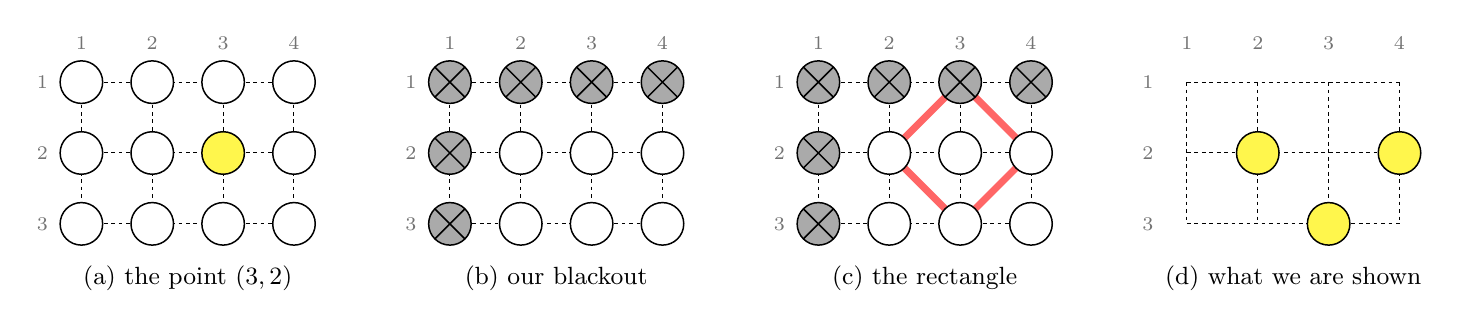
\begin{tikzpicture}[x=0.9cm,y=0.9cm,baseline=(current bounding box.north)]
  \begin{scope}[xshift=0.000cm]
    \draw[black,line width=0.36pt,dash pattern=on 1.35pt off 1.35pt] (1,-1) -- (4,-1) (1,-2) -- (4,-2) (1,-3) -- (4,-3) (1,-1) -- (1,-3) (2,-1) -- (2,-3) (3,-1) -- (3,-3) (4,-1) -- (4,-3);
    \filldraw[fill=white,draw=black,line width=0.54pt] (1,-1) circle (0.3);
    \filldraw[fill=white,draw=black,line width=0.54pt] (2,-1) circle (0.3);
    \filldraw[fill=white,draw=black,line width=0.54pt] (3,-1) circle (0.3);
    \filldraw[fill=white,draw=black,line width=0.54pt] (4,-1) circle (0.3);
    \filldraw[fill=white,draw=black,line width=0.54pt] (1,-2) circle (0.3);
    \filldraw[fill=white,draw=black,line width=0.54pt] (2,-2) circle (0.3);
    \filldraw[fill=kyellow,draw=black,line width=0.54pt] (3,-2) circle (0.3);
    \filldraw[fill=white,draw=black,line width=0.54pt] (4,-2) circle (0.3);
    \filldraw[fill=white,draw=black,line width=0.54pt] (1,-3) circle (0.3);
    \filldraw[fill=white,draw=black,line width=0.54pt] (2,-3) circle (0.3);
    \filldraw[fill=white,draw=black,line width=0.54pt] (3,-3) circle (0.3);
    \filldraw[fill=white,draw=black,line width=0.54pt] (4,-3) circle (0.3);
    \node[lab] at (1,-0.45) {1};
    \node[lab] at (2,-0.45) {2};
    \node[lab] at (3,-0.45) {3};
    \node[lab] at (4,-0.45) {4};
    \node[lab] at (0.45,-1) {1};
    \node[lab] at (0.45,-2) {2};
    \node[lab] at (0.45,-3) {3};
    \node[capt,anchor=north] at (2.50,-3.45) {(a) the point $(3,2)$};
  \end{scope}
  \begin{scope}[xshift=4.680cm]
    \draw[black,line width=0.36pt,dash pattern=on 1.35pt off 1.35pt] (1,-1) -- (4,-1) (1,-2) -- (4,-2) (1,-3) -- (4,-3) (1,-1) -- (1,-3) (2,-1) -- (2,-3) (3,-1) -- (3,-3) (4,-1) -- (4,-3);
    \filldraw[fill=kgray,draw=black,line width=0.54pt] (1,-1) circle (0.3);
    \draw[black,line width=0.54pt] (0.788,-0.788) -- (1.212,-1.212) (0.788,-1.212) -- (1.212,-0.788);
    \filldraw[fill=kgray,draw=black,line width=0.54pt] (2,-1) circle (0.3);
    \draw[black,line width=0.54pt] (1.788,-0.788) -- (2.212,-1.212) (1.788,-1.212) -- (2.212,-0.788);
    \filldraw[fill=kgray,draw=black,line width=0.54pt] (3,-1) circle (0.3);
    \draw[black,line width=0.54pt] (2.788,-0.788) -- (3.212,-1.212) (2.788,-1.212) -- (3.212,-0.788);
    \filldraw[fill=kgray,draw=black,line width=0.54pt] (4,-1) circle (0.3);
    \draw[black,line width=0.54pt] (3.788,-0.788) -- (4.212,-1.212) (3.788,-1.212) -- (4.212,-0.788);
    \filldraw[fill=kgray,draw=black,line width=0.54pt] (1,-2) circle (0.3);
    \draw[black,line width=0.54pt] (0.788,-1.788) -- (1.212,-2.212) (0.788,-2.212) -- (1.212,-1.788);
    \filldraw[fill=white,draw=black,line width=0.54pt] (2,-2) circle (0.3);
    \filldraw[fill=white,draw=black,line width=0.54pt] (3,-2) circle (0.3);
    \filldraw[fill=white,draw=black,line width=0.54pt] (4,-2) circle (0.3);
    \filldraw[fill=kgray,draw=black,line width=0.54pt] (1,-3) circle (0.3);
    \draw[black,line width=0.54pt] (0.788,-2.788) -- (1.212,-3.212) (0.788,-3.212) -- (1.212,-2.788);
    \filldraw[fill=white,draw=black,line width=0.54pt] (2,-3) circle (0.3);
    \filldraw[fill=white,draw=black,line width=0.54pt] (3,-3) circle (0.3);
    \filldraw[fill=white,draw=black,line width=0.54pt] (4,-3) circle (0.3);
    \node[lab] at (1,-0.45) {1};
    \node[lab] at (2,-0.45) {2};
    \node[lab] at (3,-0.45) {3};
    \node[lab] at (4,-0.45) {4};
    \node[lab] at (0.45,-1) {1};
    \node[lab] at (0.45,-2) {2};
    \node[lab] at (0.45,-3) {3};
    \node[capt,anchor=north] at (2.50,-3.45) {(b) our blackout};
  \end{scope}
  \begin{scope}[xshift=9.360cm]
    \draw[black,line width=0.36pt,dash pattern=on 1.35pt off 1.35pt] (1,-1) -- (4,-1) (1,-2) -- (4,-2) (1,-3) -- (4,-3) (1,-1) -- (1,-3) (2,-1) -- (2,-3) (3,-1) -- (3,-3) (4,-1) -- (4,-3);
    \draw[kred,line width=2.55pt,line join=round] (2,-2) -- (3,-1) -- (4,-2) -- (3,-3) -- cycle;
    \filldraw[fill=kgray,draw=black,line width=0.54pt] (1,-1) circle (0.3);
    \draw[black,line width=0.54pt] (0.788,-0.788) -- (1.212,-1.212) (0.788,-1.212) -- (1.212,-0.788);
    \filldraw[fill=kgray,draw=black,line width=0.54pt] (2,-1) circle (0.3);
    \draw[black,line width=0.54pt] (1.788,-0.788) -- (2.212,-1.212) (1.788,-1.212) -- (2.212,-0.788);
    \filldraw[fill=kgray,draw=black,line width=0.54pt] (3,-1) circle (0.3);
    \draw[black,line width=0.54pt] (2.788,-0.788) -- (3.212,-1.212) (2.788,-1.212) -- (3.212,-0.788);
    \filldraw[fill=kgray,draw=black,line width=0.54pt] (4,-1) circle (0.3);
    \draw[black,line width=0.54pt] (3.788,-0.788) -- (4.212,-1.212) (3.788,-1.212) -- (4.212,-0.788);
    \filldraw[fill=kgray,draw=black,line width=0.54pt] (1,-2) circle (0.3);
    \draw[black,line width=0.54pt] (0.788,-1.788) -- (1.212,-2.212) (0.788,-2.212) -- (1.212,-1.788);
    \filldraw[fill=white,draw=black,line width=0.54pt] (2,-2) circle (0.3);
    \filldraw[fill=white,draw=black,line width=0.54pt] (3,-2) circle (0.3);
    \filldraw[fill=white,draw=black,line width=0.54pt] (4,-2) circle (0.3);
    \filldraw[fill=kgray,draw=black,line width=0.54pt] (1,-3) circle (0.3);
    \draw[black,line width=0.54pt] (0.788,-2.788) -- (1.212,-3.212) (0.788,-3.212) -- (1.212,-2.788);
    \filldraw[fill=white,draw=black,line width=0.54pt] (2,-3) circle (0.3);
    \filldraw[fill=white,draw=black,line width=0.54pt] (3,-3) circle (0.3);
    \filldraw[fill=white,draw=black,line width=0.54pt] (4,-3) circle (0.3);
    \node[lab] at (1,-0.45) {1};
    \node[lab] at (2,-0.45) {2};
    \node[lab] at (3,-0.45) {3};
    \node[lab] at (4,-0.45) {4};
    \node[lab] at (0.45,-1) {1};
    \node[lab] at (0.45,-2) {2};
    \node[lab] at (0.45,-3) {3};
    \node[capt,anchor=north] at (2.50,-3.45) {(c) the rectangle};
  \end{scope}
  \begin{scope}[xshift=14.040cm]
    \draw[black,line width=0.36pt,dash pattern=on 1.35pt off 1.35pt] (1,-1) -- (4,-1) (1,-2) -- (4,-2) (1,-3) -- (4,-3) (1,-1) -- (1,-3) (2,-1) -- (2,-3) (3,-1) -- (3,-3) (4,-1) -- (4,-3);
    \filldraw[fill=kyellow,draw=black,line width=0.54pt] (2,-2) circle (0.3);
    \filldraw[fill=kyellow,draw=black,line width=0.54pt] (4,-2) circle (0.3);
    \filldraw[fill=kyellow,draw=black,line width=0.54pt] (3,-3) circle (0.3);
    \node[lab] at (1,-0.45) {1};
    \node[lab] at (2,-0.45) {2};
    \node[lab] at (3,-0.45) {3};
    \node[lab] at (4,-0.45) {4};
    \node[lab] at (0.45,-1) {1};
    \node[lab] at (0.45,-2) {2};
    \node[lab] at (0.45,-3) {3};
    \node[capt,anchor=north] at (2.50,-3.45) {(d) what we are shown};
  \end{scope}
\end{tikzpicture}
}
\caption{One round on a largest valid blackout of the $3\times4$ grid. Points are
(column, row). Gray crossed circles are black. Panel (c) shows the red rectangle,
and (d) its yellow corners. The three yellow corners fix the fourth by
Lemma~\ref{lem:threecorners}.}
\label{fig:game}
\end{figure}

Write $f(h,m)$ for the largest size of a valid blackout, and $a_h(m)$ for the
number of valid blackouts of that size. We call them \emph{optima}. The
values $f(h,m)$ form the table \seqnum{A397315} of the OEIS~\cite{oeis}, and
the counts $a_h(m)$ form the table \seqnum{A399580}. The companion
paper~\cite{pemmasaniExtremal} is about $f$. It proves the bound
$f(h,m)\le m+\lfloor h^2/4\rfloor$ with its cases of equality, shows that
equality holds for all large $m$, finds the order of the least such width, and
gives $f(h,m)$ for every $h\le6$. This paper is about the counts. It uses from
the companion paper only the statements listed in Theorem~\ref{thm:imports},
and the companion paper uses nothing from this one.

Put $q_h=\lfloor h^2/4\rfloor$. We record a blackout by the set of black rows
of each column, read from left to right. The results are as follows.

\begin{enumerate}[(1),leftmargin=*]
\item \emph{Two rows.} We have $a_2(m)=m2^{m-1}$ for $m\ge3$ (\seqnum{A001787}).
Up to symmetry the optima are counted by \seqnum{A322284}, by a bijection with
placements of kings (Theorem~\ref{thm:strip} and Proposition~\ref{prop:kings}).
\item \emph{Three rows.} We find $a_3(m)$ in closed form
(Theorem~\ref{thm:threecount}). For $m\ge4$ it is $4(m-1)(3m+2)\,3^{m-5}+E_m$,
where $E_m$ counts the optima with a column black in rows $1$ and $3$ and has
order $m^2(1+\sqrt3)^m$. So $a_3(m)\sim\frac4{81}m^23^m$. These sequences are
\seqnum{A401223} and \seqnum{A398448}. The series $\sum_{m\ge1}a_3(m)z^m$ is
rational with denominator $(1-3z)^3(1-2z-2z^2)^3(1+2z^2)^3$
(Theorem~\ref{thm:threegf}). The optima up to symmetry are counted in
Theorem~\ref{thm:threeorbits}, which gives \seqnum{A401226}.
\item \emph{Four rows.} For $m\ge4$ no valid blackout hides all $4$ corners of a
rectangle (Theorem~\ref{thm:hidden}). For $m\ge6$ a finite automaton with $6$
columns of memory accepts exactly the optima
(Proposition~\ref{prop:fourautomaton}). With computer help we find the generating function of $a_4(m)$
(\seqnum{A401224}). It is rational with a reduced denominator of degree $420$, and
$a_4(m)\sim c\,m^4\rho_4^m$, where $\rho_4=3.35199\ldots$ is algebraic of
degree $20$ (Theorem~\ref{thm:fourgfexact} and Corollary~\ref{cor:fourgrowth}).
\item \emph{Five rows.} Two transfer counters give $a_5(m)$ for $8\le m\le23$
(\seqnum{A401225}, Table~\ref{tab:fivevalues}).
\item \emph{Fixed height.} For every $h$ the valid column words form a regular
language, $f(h,m)-m$ is ultimately periodic in $m$, and $\sum_{m\ge1}a_h(m)z^m$
is rational (Theorems~\ref{thm:regular} and~\ref{thm:rational}). The proof does
not use the companion paper.
\item \emph{Tilted rectangles.} A tilted lattice rectangle whose bounding box has
height $n$ has width at most $\lfloor n^2/4\rfloor+1$. This proves a conjecture
of Kagey in \seqnum{A338885}, that the largest entry of its row $n$ is
\seqnum{A033638}$(n)$ (Remark~\ref{cor:oeisconj}).
\end{enumerate}

Statements that rest on a computation are marked as computer-assisted, and
Section~\ref{sec:verify} names the programs and the stored evidence.

\paragraph{Related work.} The value $f(3,m)=m+2$ was also proved
in Lean by the Omega Institute~\cite{trureturing2026}. The row bound
$f(h,m)\le m+q_h$ of the companion paper is, in graph form, due to
Neuwirth~\cite[Theorem~1(ii) and Proposition~17]{neuwirth2001}. Counting
configurations on a grid of fixed height by a transfer matrix is a standard
method~\cite[Section~4.7]{stanley2012}, \cite[Proposition~V.6]{flajolet2009}.
Examples are the independent sets of grid
graphs~\cite{calkinwilf1998,euler2005}, the nonattacking kings of
Wilf~\cite{wilf1995}, and the dominating sets of grids and king graphs counted
by Mertens~\cite{mertens2024}.

\section{Definitions and tools}\label{sec:setup}

\subsection{Blackouts}

An $h\times m$ grid has $h$ rows, $m$ columns, and point set $V$. The point
$(i,j)$ lies in column $i$ and row $j$, with $(1,1)$ at the top left
(Figure~\ref{fig:game}(a)). A \emph{rectangle} has four grid points as corners
and positive area. We write $C(R)$ for the corner set of a rectangle $R$. It is
\emph{axis-aligned} if its sides follow the grid lines, and \emph{tilted}
otherwise.

A \emph{blackout} is a set $S\subseteq V$ of black points. The other points are
white. The \emph{presentation} of a rectangle $R$ is $\pres(R)=C(R)\setminus S$,
the set of its white corners. We say that $R$ \emph{shows} these corners, and
that $R$ is \emph{hidden} if it shows none.

\begin{definition}[valid blackout]\label{def:valid}
A blackout $S$ is \emph{valid} if distinct rectangles have distinct
presentations. We write $f(h,m)$ for the largest size of a valid blackout
of the $h\times m$ grid, and $a_h(m)$ for the number of valid blackouts of that
size, which we call \emph{optima}. We count them as sets of points, so
reflections and rotations are not identified.
\end{definition}

Transposing the grid gives $f(h,m)=f(m,h)$ and $a_h(m)=a_m(h)$. A grid with
$1$ row or $1$ column has no rectangles, so $f(1,m)=m$ and $a_1(m)=1$.

Column $i$ of a blackout has \emph{black rows} $B_i=\{j:(i,j)\in S\}$. It is
\emph{empty}, a \emph{singleton}, a \emph{double}, or a \emph{triple} when
$|B_i|$ is $0$, $1$, $2$, or $3$, and \emph{full} when $|B_i|=h$. The \emph{column
word} of $S$ is $B_1B_2\cdots B_m$. The \emph{pair set} $F$ of $S$ is the set of
pairs of rows that are both black in some column. Throughout,
$q_h=\lfloor h^2/4\rfloor$, which is \seqnum{A002620}$(h)$.

\begin{lemma}[difference sets]\label{lem:diff}
Two rectangles $R_1$ and $R_2$ have the same presentation if and only if
$C(R_1)\triangle C(R_2)\subseteq S$.
\end{lemma}

\begin{proof}
The sets $C(R_1)\setminus S$ and $C(R_2)\setminus S$ agree exactly when every
point that lies in just one of $C(R_1)$ and $C(R_2)$ belongs to $S$.
\end{proof}

\begin{lemma}[three corners suffice]\label{lem:threecorners}
Three corners of a rectangle determine it. Hence two distinct rectangles with the
same presentation show at most $2$ corners, and a valid blackout hides at most
$1$ rectangle.
\end{lemma}

\begin{proof}
Three corners form a right triangle. Its right angle is at the corner $q$
adjacent to the other two, $p$ and $r$, so the fourth corner is $p+r-q$. Two
hidden rectangles would both have the empty presentation.
\end{proof}

\subsection{Tilted rectangles}

Put $W_h=1+\lfloor(h-1)^2/4\rfloor$, so $W_3=2$, $W_4=3$, and $W_5=5$.

\begin{lemma}[leftmost corner]\label{lem:leftmost}
A tilted rectangle $R$ has a unique corner $\ell=(x,r)$ in its smallest column.
The sides from $\ell$ are $(a,-b)$ and $(c,d)$ with positive integers $a,b,c,d$
and $ac=bd$, and the corners are
\begin{equation}\label{eq:tilt-param}
(x,r),\qquad(x+a,\,r-b),\qquad(x+c,\,r+d),\qquad(x+a+c,\,r-b+d).
\end{equation}
The rectangle meets the rows $r-b$ to $r+d$ and the columns $x$ to $x+a+c$. We
call $a+c$ its \emph{span}.
\end{lemma}

\begin{proof}
No side of $R$ is vertical. Hence two corners in the smallest column $x$ would
be opposite. The other two corners have the same midpoint, so they would also
lie in column $x$, and $R$ would have no area. The two sides from
$\ell$ therefore have positive first coordinates $a$ and $c$. They are
perpendicular, so their second coordinates have product $-ac$. Thus one
side points up and the other down, which gives the form above with $ac=bd$.
\end{proof}

\begin{lemma}[span bound]\label{lem:span}
Every tilted rectangle of the $h\times m$ grid has span $a+c\le W_h$.
\end{lemma}

\begin{proof}
The rectangle fits in $h$ rows, so $b+d\le h-1$. Since $(a-1)(c-1)\ge0$, we get
$a+c\le ac+1=bd+1$. Finally $bd\le\lfloor(b+d)^2/4\rfloor\le W_h-1$.
\end{proof}

\begin{remark}[a conjecture in \seqnum{A338885}]\label{cor:oeisconj}
The same computation settles a conjecture of Kagey. Row $n$ of his triangle
\seqnum{A338885} lists all $k$ such that some tilted lattice rectangle touches
all $4$ sides of an $n\times k$ rectangle, and he conjectures there that the
largest such $k$ is \seqnum{A033638}$(n)=\lfloor n^2/4\rfloor+1$. This is true
for every $n\ge2$. In~\eqref{eq:tilt-param} the bounding box has height $b+d=n$
and width $k=a+c$. As in Lemma~\ref{lem:span}, $k\le bd+1\le\lfloor n^2/4\rfloor+1$.
For equality take $b=\lfloor n/2\rfloor$, $d=\lceil n/2\rceil$, and the
perpendicular sides $(1,-b)$ and $(bd,d)$.
\end{remark}

The \emph{diamond} $D(i,j)$ is the square with corners $(i,j+1)$, $(i+1,j)$,
$(i+2,j+1)$, and $(i+1,j+2)$. The rectangles $\kA_i$, $\kB_i$, $\kC_i$, and
$\kE_i$ have one corner in each of the columns $i$ to $i+3$, in the rows
$3412$, $3142$, $2413$, and $2143$ from left to right (Figure~\ref{fig:tilted}).

\begin{figure}[t]
\centering
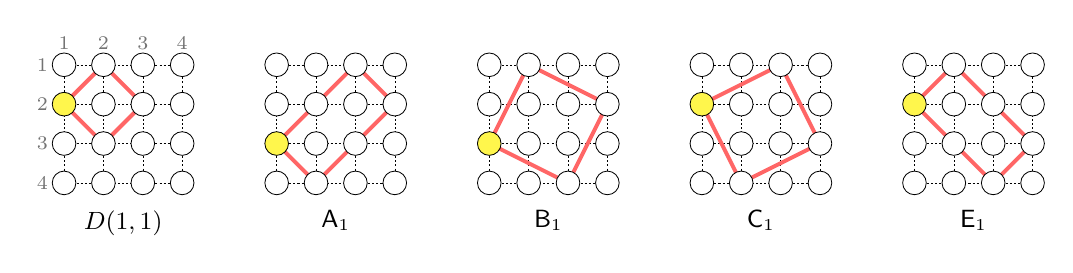
\begin{tikzpicture}[x=0.5cm,y=0.5cm,baseline=(current bounding box.north)]
  \begin{scope}[xshift=0.000cm]
    \draw[black,line width=0.20pt,dash pattern=on 0.75pt off 0.75pt] (1,-1) -- (4,-1) (1,-2) -- (4,-2) (1,-3) -- (4,-3) (1,-4) -- (4,-4) (1,-1) -- (1,-4) (2,-1) -- (2,-4) (3,-1) -- (3,-4) (4,-1) -- (4,-4);
    \draw[kred,line width=1.42pt,line join=round] (1,-2) -- (2,-1) -- (3,-2) -- (2,-3) -- cycle;
    \filldraw[fill=white,draw=black,line width=0.30pt] (1,-1) circle (0.3);
    \filldraw[fill=white,draw=black,line width=0.30pt] (2,-1) circle (0.3);
    \filldraw[fill=white,draw=black,line width=0.30pt] (3,-1) circle (0.3);
    \filldraw[fill=white,draw=black,line width=0.30pt] (4,-1) circle (0.3);
    \filldraw[fill=kyellow,draw=black,line width=0.30pt] (1,-2) circle (0.3);
    \filldraw[fill=white,draw=black,line width=0.30pt] (2,-2) circle (0.3);
    \filldraw[fill=white,draw=black,line width=0.30pt] (3,-2) circle (0.3);
    \filldraw[fill=white,draw=black,line width=0.30pt] (4,-2) circle (0.3);
    \filldraw[fill=white,draw=black,line width=0.30pt] (1,-3) circle (0.3);
    \filldraw[fill=white,draw=black,line width=0.30pt] (2,-3) circle (0.3);
    \filldraw[fill=white,draw=black,line width=0.30pt] (3,-3) circle (0.3);
    \filldraw[fill=white,draw=black,line width=0.30pt] (4,-3) circle (0.3);
    \filldraw[fill=white,draw=black,line width=0.30pt] (1,-4) circle (0.3);
    \filldraw[fill=white,draw=black,line width=0.30pt] (2,-4) circle (0.3);
    \filldraw[fill=white,draw=black,line width=0.30pt] (3,-4) circle (0.3);
    \filldraw[fill=white,draw=black,line width=0.30pt] (4,-4) circle (0.3);
    \node[lab] at (1,-0.45) {1};
    \node[lab] at (2,-0.45) {2};
    \node[lab] at (3,-0.45) {3};
    \node[lab] at (4,-0.45) {4};
    \node[lab] at (0.45,-1) {1};
    \node[lab] at (0.45,-2) {2};
    \node[lab] at (0.45,-3) {3};
    \node[lab] at (0.45,-4) {4};
    \node[capt,anchor=north] at (2.50,-4.45) {$D(1,1)$};
  \end{scope}
  \begin{scope}[xshift=2.700cm]
    \draw[black,line width=0.20pt,dash pattern=on 0.75pt off 0.75pt] (1,-1) -- (4,-1) (1,-2) -- (4,-2) (1,-3) -- (4,-3) (1,-4) -- (4,-4) (1,-1) -- (1,-4) (2,-1) -- (2,-4) (3,-1) -- (3,-4) (4,-1) -- (4,-4);
    \draw[kred,line width=1.42pt,line join=round] (1,-3) -- (2,-4) -- (4,-2) -- (3,-1) -- cycle;
    \filldraw[fill=white,draw=black,line width=0.30pt] (1,-1) circle (0.3);
    \filldraw[fill=white,draw=black,line width=0.30pt] (2,-1) circle (0.3);
    \filldraw[fill=white,draw=black,line width=0.30pt] (3,-1) circle (0.3);
    \filldraw[fill=white,draw=black,line width=0.30pt] (4,-1) circle (0.3);
    \filldraw[fill=white,draw=black,line width=0.30pt] (1,-2) circle (0.3);
    \filldraw[fill=white,draw=black,line width=0.30pt] (2,-2) circle (0.3);
    \filldraw[fill=white,draw=black,line width=0.30pt] (3,-2) circle (0.3);
    \filldraw[fill=white,draw=black,line width=0.30pt] (4,-2) circle (0.3);
    \filldraw[fill=kyellow,draw=black,line width=0.30pt] (1,-3) circle (0.3);
    \filldraw[fill=white,draw=black,line width=0.30pt] (2,-3) circle (0.3);
    \filldraw[fill=white,draw=black,line width=0.30pt] (3,-3) circle (0.3);
    \filldraw[fill=white,draw=black,line width=0.30pt] (4,-3) circle (0.3);
    \filldraw[fill=white,draw=black,line width=0.30pt] (1,-4) circle (0.3);
    \filldraw[fill=white,draw=black,line width=0.30pt] (2,-4) circle (0.3);
    \filldraw[fill=white,draw=black,line width=0.30pt] (3,-4) circle (0.3);
    \filldraw[fill=white,draw=black,line width=0.30pt] (4,-4) circle (0.3);
    \node[capt,anchor=north] at (2.50,-4.45) {$\kA_1$};
  \end{scope}
  \begin{scope}[xshift=5.400cm]
    \draw[black,line width=0.20pt,dash pattern=on 0.75pt off 0.75pt] (1,-1) -- (4,-1) (1,-2) -- (4,-2) (1,-3) -- (4,-3) (1,-4) -- (4,-4) (1,-1) -- (1,-4) (2,-1) -- (2,-4) (3,-1) -- (3,-4) (4,-1) -- (4,-4);
    \draw[kred,line width=1.42pt,line join=round] (1,-3) -- (3,-4) -- (4,-2) -- (2,-1) -- cycle;
    \filldraw[fill=white,draw=black,line width=0.30pt] (1,-1) circle (0.3);
    \filldraw[fill=white,draw=black,line width=0.30pt] (2,-1) circle (0.3);
    \filldraw[fill=white,draw=black,line width=0.30pt] (3,-1) circle (0.3);
    \filldraw[fill=white,draw=black,line width=0.30pt] (4,-1) circle (0.3);
    \filldraw[fill=white,draw=black,line width=0.30pt] (1,-2) circle (0.3);
    \filldraw[fill=white,draw=black,line width=0.30pt] (2,-2) circle (0.3);
    \filldraw[fill=white,draw=black,line width=0.30pt] (3,-2) circle (0.3);
    \filldraw[fill=white,draw=black,line width=0.30pt] (4,-2) circle (0.3);
    \filldraw[fill=kyellow,draw=black,line width=0.30pt] (1,-3) circle (0.3);
    \filldraw[fill=white,draw=black,line width=0.30pt] (2,-3) circle (0.3);
    \filldraw[fill=white,draw=black,line width=0.30pt] (3,-3) circle (0.3);
    \filldraw[fill=white,draw=black,line width=0.30pt] (4,-3) circle (0.3);
    \filldraw[fill=white,draw=black,line width=0.30pt] (1,-4) circle (0.3);
    \filldraw[fill=white,draw=black,line width=0.30pt] (2,-4) circle (0.3);
    \filldraw[fill=white,draw=black,line width=0.30pt] (3,-4) circle (0.3);
    \filldraw[fill=white,draw=black,line width=0.30pt] (4,-4) circle (0.3);
    \node[capt,anchor=north] at (2.50,-4.45) {$\kB_1$};
  \end{scope}
  \begin{scope}[xshift=8.100cm]
    \draw[black,line width=0.20pt,dash pattern=on 0.75pt off 0.75pt] (1,-1) -- (4,-1) (1,-2) -- (4,-2) (1,-3) -- (4,-3) (1,-4) -- (4,-4) (1,-1) -- (1,-4) (2,-1) -- (2,-4) (3,-1) -- (3,-4) (4,-1) -- (4,-4);
    \draw[kred,line width=1.42pt,line join=round] (1,-2) -- (2,-4) -- (4,-3) -- (3,-1) -- cycle;
    \filldraw[fill=white,draw=black,line width=0.30pt] (1,-1) circle (0.3);
    \filldraw[fill=white,draw=black,line width=0.30pt] (2,-1) circle (0.3);
    \filldraw[fill=white,draw=black,line width=0.30pt] (3,-1) circle (0.3);
    \filldraw[fill=white,draw=black,line width=0.30pt] (4,-1) circle (0.3);
    \filldraw[fill=kyellow,draw=black,line width=0.30pt] (1,-2) circle (0.3);
    \filldraw[fill=white,draw=black,line width=0.30pt] (2,-2) circle (0.3);
    \filldraw[fill=white,draw=black,line width=0.30pt] (3,-2) circle (0.3);
    \filldraw[fill=white,draw=black,line width=0.30pt] (4,-2) circle (0.3);
    \filldraw[fill=white,draw=black,line width=0.30pt] (1,-3) circle (0.3);
    \filldraw[fill=white,draw=black,line width=0.30pt] (2,-3) circle (0.3);
    \filldraw[fill=white,draw=black,line width=0.30pt] (3,-3) circle (0.3);
    \filldraw[fill=white,draw=black,line width=0.30pt] (4,-3) circle (0.3);
    \filldraw[fill=white,draw=black,line width=0.30pt] (1,-4) circle (0.3);
    \filldraw[fill=white,draw=black,line width=0.30pt] (2,-4) circle (0.3);
    \filldraw[fill=white,draw=black,line width=0.30pt] (3,-4) circle (0.3);
    \filldraw[fill=white,draw=black,line width=0.30pt] (4,-4) circle (0.3);
    \node[capt,anchor=north] at (2.50,-4.45) {$\kC_1$};
  \end{scope}
  \begin{scope}[xshift=10.800cm]
    \draw[black,line width=0.20pt,dash pattern=on 0.75pt off 0.75pt] (1,-1) -- (4,-1) (1,-2) -- (4,-2) (1,-3) -- (4,-3) (1,-4) -- (4,-4) (1,-1) -- (1,-4) (2,-1) -- (2,-4) (3,-1) -- (3,-4) (4,-1) -- (4,-4);
    \draw[kred,line width=1.42pt,line join=round] (1,-2) -- (3,-4) -- (4,-3) -- (2,-1) -- cycle;
    \filldraw[fill=white,draw=black,line width=0.30pt] (1,-1) circle (0.3);
    \filldraw[fill=white,draw=black,line width=0.30pt] (2,-1) circle (0.3);
    \filldraw[fill=white,draw=black,line width=0.30pt] (3,-1) circle (0.3);
    \filldraw[fill=white,draw=black,line width=0.30pt] (4,-1) circle (0.3);
    \filldraw[fill=kyellow,draw=black,line width=0.30pt] (1,-2) circle (0.3);
    \filldraw[fill=white,draw=black,line width=0.30pt] (2,-2) circle (0.3);
    \filldraw[fill=white,draw=black,line width=0.30pt] (3,-2) circle (0.3);
    \filldraw[fill=white,draw=black,line width=0.30pt] (4,-2) circle (0.3);
    \filldraw[fill=white,draw=black,line width=0.30pt] (1,-3) circle (0.3);
    \filldraw[fill=white,draw=black,line width=0.30pt] (2,-3) circle (0.3);
    \filldraw[fill=white,draw=black,line width=0.30pt] (3,-3) circle (0.3);
    \filldraw[fill=white,draw=black,line width=0.30pt] (4,-3) circle (0.3);
    \filldraw[fill=white,draw=black,line width=0.30pt] (1,-4) circle (0.3);
    \filldraw[fill=white,draw=black,line width=0.30pt] (2,-4) circle (0.3);
    \filldraw[fill=white,draw=black,line width=0.30pt] (3,-4) circle (0.3);
    \filldraw[fill=white,draw=black,line width=0.30pt] (4,-4) circle (0.3);
    \node[capt,anchor=north] at (2.50,-4.45) {$\kE_1$};
  \end{scope}
\end{tikzpicture}

\caption{The tilted rectangles of the $4\times m$ grid, up to translation. Each is
drawn in a $4\times4$ window, and its leftmost corner $\ell$ is yellow.}
\label{fig:tilted}
\end{figure}

\begin{lemma}[tilted rectangles on $3$ and $4$ rows]\label{lem:tilted-narrow}
The tilted rectangles of the $3\times m$ grid are the diamonds $D(i,1)$. Those of
the $4\times m$ grid are $D(i,1)$, $D(i,2)$, $\kA_i$, $\kB_i$, $\kC_i$, and
$\kE_i$.
\end{lemma}

\begin{proof}
We use Lemma~\ref{lem:leftmost}. On $3$ rows, $b+d\le2$ forces $b=d=1$. Then
$ac=1$, so $a=c=1$ and $\ell$ is in row $2$. On $4$ rows, $b=d=1$ again gives
diamonds, with $\ell$ in row $2$ or $3$. Otherwise $\{b,d\}=\{1,2\}$. Then
$ac=2$, so $\{a,c\}=\{1,2\}$, and $\ell$ is in row $1+b$. The $4$ choices of
sides, $(2,-2),(1,1)$, $(1,-2),(2,1)$, $(2,-1),(1,2)$, and $(1,-1),(2,2)$,
give $\kA_i$, $\kB_i$, $\kC_i$, and $\kE_i$.
\end{proof}

\subsection{Axis-aligned rectangles}

A blackout $S$ is \emph{axis-valid} if distinct axis-aligned rectangles have
distinct presentations. In the \emph{row-column graph} $G_S$, the vertices are
the rows $r_1,\dots,r_h$ and the columns $c_1,\dots,c_m$, and $r_j$ is joined to
$c_i$ for each black point $(i,j)$.

\begin{lemma}[short cycles]\label{lem:girth}
If $G_S$ has no $4$-cycle and no $6$-cycle, then $S$ is axis-valid. The converse
holds for $m\ge3$.
\end{lemma}

\begin{proof}
Let $m\ge3$. A $4$-cycle $r_j\,c_i\,r_{j'}\,c_{i'}$ gives the rectangles
$\{i,w\}\times\{j,j'\}$ and $\{i',w\}\times\{j,j'\}$ for a third column $w$.
Their corner sets differ in $4$ black points. A $6$-cycle
$r_a\,c_x\,r_b\,c_y\,r_c\,c_z$ gives $\{x,y\}\times\{a,b\}$ and
$\{y,z\}\times\{a,c\}$, whose corner sets differ in the $6$ black points of the
cycle. In both cases Lemma~\ref{lem:diff} shows that $S$ is not axis-valid.

Conversely, let axis-aligned rectangles $R_1\ne R_2$ have the same presentation,
so that $C(R_1)\triangle C(R_2)\subseteq S$. They do not share opposite corners.
Hence they share $0$, $1$, or $2$ corners, and $2$ shared corners lie in one row
or in one column. We may assume that it is a row $a$. If they share no corner,
then $R_1$ is hidden, which is a $4$-cycle. If they share $(x,a)$ and $(y,a)$,
their other rows $b\ne c$ give the $4$-cycle $r_b\,c_x\,r_c\,c_y$. If they share
just $(x,a)$, write $R_1=\{x,y\}\times\{a,b\}$ and $R_2=\{x,z\}\times\{a,c\}$
with $y\ne z$ and $b\ne c$. The other $6$ corners are black and form the
$6$-cycle $r_a\,c_y\,r_b\,c_x\,r_c\,c_z$.
\end{proof}

The next lemma tells when a set of at most $2$ points is the presentation of
an axis-aligned rectangle.

\begin{lemma}[axis-aligned rivals]\label{lem:rival}
Let $S$ hide no axis-aligned rectangle, and let $P$ be a set of at most $2$
white points. A \emph{rival} of $P$ is an axis-aligned rectangle with
presentation $P$. The empty set has no rival. Otherwise $P$ has a rival exactly
in the following cases.
\begin{enumerate}[(a)]
\item $P=\{(x,r)\}$, and some $s\in B_x$ has $\{r,s\}\in F$.
\item $P=\{(x,r),(x,s)\}$ is a vertical pair, and $\{r,s\}\in F$.
\item $P=\{(x,r),(z,r)\}$ is a horizontal pair, and $B_x\cap B_z\ne\emptyset$.
\item $P=\{(x,r),(z,s)\}$ is an oblique pair with $x\ne z$ and $r\ne s$, and
$(x,s)$ and $(z,r)$ are black.
\end{enumerate}
\end{lemma}

\begin{proof}
A rival of $P\ne\emptyset$ has rows $\{r,s\}$ and columns $\{x,z\}$, and each of
its corners outside $P$ is black. Reading off these corners gives the $4$
conditions. In (a) the black corners are $(x,s)$, $(z,r)$, and $(z,s)$, so
$s\in B_x$ and column $z$ contains the pair $\{r,s\}$. Here $z\ne x$ holds
automatically, since $(x,r)$ is white.
\end{proof}

\subsection{What we use from the companion paper}

\begin{theorem}[{\cite{pemmasaniExtremal}}]\label{thm:imports}
Let $m\ge3$.
\begin{enumerate}[(a)]
\item \textup{(Row bound.)} Every axis-valid blackout of the $h\times m$ grid has
at most $m+q_h$ points. Hence $f(h,m)\le m+q_h$.
\item \textup{(Equality.)} Let $h\ge4$. A blackout of the $h\times m$ grid with
$m+q_h$ points is axis-valid if and only if every column is a singleton or a
double, the $q_h$ doubles have distinct row pairs, and these pairs are the edges
of a complete bipartite graph on the rows with parts of sizes $\lfloor h/2\rfloor$
and $\lceil h/2\rceil$.
\item \textup{(Values.)} We have $f(2,m)=m+1$ and $f(3,m)=m+2$. We have
$f(4,4)=7$, $f(4,5)=8$, and $f(4,m)=m+4$ for $m\ge6$. We have $f(5,5)=10$,
$f(5,6)=11$, $f(5,7)=12$, and $f(5,m)=m+6$ for $m\ge8$.
\end{enumerate}
\end{theorem}

In the companion paper the values $f(4,4)$, $f(4,5)$, $f(5,6)$, and $f(5,7)$
rest on computer searches, and $f(5,m)=m+6$ rests on a finite check that is
also verified in Lean. We do not need (c) for $2$ and $3$ rows, since
Theorem~\ref{thm:strip} and Corollary~\ref{cor:threevalue} prove these cases
again. Table~\ref{tab:values} lists $f(h,m)$ and $a_h(m)$ for $h\le5$.

\begin{table}[!htb]
\centering\footnotesize\setlength{\tabcolsep}{4pt}
\begin{tabular}{@{}r|rrrr@{}}
\multicolumn{5}{c}{$f(h,m)$}\\
\toprule
$m\backslash h$ & $2$ & $3$ & $4$ & $5$\\
\midrule
$2$ & $4$ & $4$ & $5$ & $6$\\
$3$ & $4$ & $5$ & $6$ & $7$\\
$4$ & $5$ & $6$ & $7$ & $8$\\
$5$ & $6$ & $7$ & $8$ & $10$\\
$6$ & $7$ & $8$ & $10$ & $11$\\
$7$ & $8$ & $9$ & $11$ & $12$\\
$8$ & $9$ & $10$ & $12$ & $14$\\
$9$ & $10$ & $11$ & $13$ & $15$\\
$10$ & $11$ & $12$ & $14$ & $16$\\
$11$ & $12$ & $13$ & $15$ & $17$\\
$12$ & $13$ & $14$ & $16$ & $18$\\
$13$ & $14$ & $15$ & $17$ & $19$\\
\bottomrule
\end{tabular}\hspace{1.2em}
\begin{tabular}{@{}r|rrrr@{}}
\multicolumn{5}{c}{$a_h(m)$}\\
\toprule
$m\backslash h$ & $2$ & $3$ & $4$ & $5$\\
\midrule
$2$ & $1$ & $12$ & $32$ & $80$\\
$3$ & $12$ & $53$ & $224$ & $892$\\
$4$ & $32$ & $224$ & $316$ & $1810$\\
$5$ & $80$ & $892$ & $1810$ & $8$\\
$6$ & $192$ & $3420$ & $26$ & $76$\\
$7$ & $448$ & $12704$ & $292$ & $1184$\\
$8$ & $1024$ & $45864$ & $2118$ & $4$\\
$9$ & $2304$ & $161992$ & $13332$ & $44$\\
$10$ & $5120$ & $562912$ & $75398$ & $350$\\
$11$ & $11264$ & $1930312$ & $402656$ & $3004$\\
$12$ & $24576$ & $6545496$ & $2037848$ & $24706$\\
$13$ & $53248$ & $21988784$ & $9894016$ & $193406$\\
\bottomrule
\end{tabular}
\caption{The values of $f(h,m)$ (\seqnum{A397315}) and $a_h(m)$
(\seqnum{A399580}) for $h\le5$. The columns $h=2$, $3$, $4$ of the counts are
\seqnum{A001787} from $m=3$, \seqnum{A401223}, and \seqnum{A401224}, and the
column $h=5$ is \seqnum{A401225} from $m=8$. The counts $a_4(m)$ and $a_5(m)$ with
$m\ge4$ are computer-assisted.}
\label{tab:values}
\end{table}

\section{Two rows}\label{sec:strip}

On $2$ rows every rectangle is axis-aligned, since a tilted rectangle meets at
least $3$ rows by Lemma~\ref{lem:leftmost}. A rectangle of the $2\times m$ grid
is therefore given by its $2$ columns.

\begin{theorem}[Strip Theorem]\label{thm:strip}
Let $m\ge3$.
\begin{enumerate}[(a)]
\item A blackout of the $2\times m$ grid is valid if and only if at most $1$ of
its columns is full.
\item We have $f(2,m)=m+1$, and the optima are the blackouts with $1$ full column
and $1$ black point in every other column.
\item We have $a_2(m)=m\,2^{m-1}$. So row $2$ of \seqnum{A399580} is
\seqnum{A001787} from $m=3$ on.
\end{enumerate}
For $m=2$ there is $1$ rectangle, so $f(2,2)=4$ and $a_2(2)=1$.
\end{theorem}

\begin{proof}
(a) Take two distinct rectangles, with column sets $\{p,q\}$ and $\{p',q'\}$.
Their corner sets differ exactly in the points of the columns that belong to
one of these sets and not to the other. There are $2$ or $4$ such columns.
Conversely, for any two columns $p\ne q$ choose a third column $w$. Here we
use $m\ge3$. The rectangles on $\{w,p\}$ and $\{w,q\}$ differ exactly in
the points of columns $p$ and $q$. By Lemma~\ref{lem:diff}, a blackout is
valid if and only if no $2$ columns are full.

(b, c) A valid blackout keeps a white point in all but at most $1$ column, so
$|S|\le2m-(m-1)=m+1$. Equality requires $1$ full column and exactly $1$ black
point in each other column. There are $m$ choices for the full column and $2$
choices in each of the other $m-1$ columns.
\end{proof}

The $2\times m$ grid has $4$ symmetries, generated by the row reflection and
the column reversal. We count the optima up to these.

\begin{proposition}[orbits and kings]\label{prop:kings}
For $m\ge3$ the number of optima of the $2\times m$ grid up to symmetry is
\[
m\,2^{m-3}+[m\text{ odd}]\,2^{(m-3)/2}.
\]
It equals \seqnum{A322284}$(m-1)$, the number of ways to place $m-1$
nonattacking kings on a $2\times(2m-2)$ board up to symmetry.
\end{proposition}

\begin{proof}
We use Burnside's lemma. The identity fixes all $m2^{m-1}$ optima, and the row
reflection fixes none, since it moves every singleton. The column reversal and
the half turn can fix an optimum only when $m$ is odd and the full column is
the middle one. Each of them then fixes $2^{(m-1)/2}$ optima, since the
singleton columns come in mirror pairs and one column of each pair determines
the other. Dividing the sum by $4$ gives the formula.

For the kings, put $n=m-1$. Two kings on a board with $2$ rows attack each other
exactly when their columns are equal or adjacent. So a placement of $n$
nonattacking kings on the $2\times2n$ board consists of columns
$c_1<\cdots<c_n$ with $c_{j+1}\ge c_j+2$, and a row $r_j$ for each king. The
numbers $c_1-1$, $c_{j+1}-c_j-2$ for $1\le j<n$, and $2n-c_n$ are nonnegative and
sum to $1$. Hence exactly one of these $n+1$ numbers is $1$. If it is the $e$th,
then $c_j=2j-1+[j\ge e]$. Send this placement to the optimum with full column
$e$ and singleton rows $r_1,\ldots,r_n$ from left to right. This is a bijection.
It commutes with the row reflection. The column reversal of the board sends
$c$ to $2n+1-c$ and reverses the order of the rows $r_j$. Since
$2n+1-c_{n+1-j}=2j-1+[j\ge n+2-e]$, it sends $e$ to $n+2-e=m+1-e$, as the column
reversal of the grid does. Hence the orbits correspond.
\end{proof}

\section{Three rows}\label{sec:three}

Take $m\ge3$ and number the rows $1,2,3$ downward. We write a column as a
letter. The singletons are $a=\{1\}$, $b=\{2\}$, and $c=\{3\}$, the doubles are
$A=\{1,2\}$, $B=\{1,3\}$, and $C=\{2,3\}$, and the triple is $X=\{1,2,3\}$. We
call $a$ and $c$ the \emph{outer} letters. A blackout without empty columns is
then a word in these $7$ letters. We also write $A$, $B$, $C$ for the
corresponding pairs of rows, so that the pair set $F$ is a set of letters.

\subsection{The candidates and the window rules}

\begin{proposition}[the two types]\label{prop:threeclass}
Let $m\ge3$.
\begin{enumerate}[(a)]
\item A valid blackout of the $3\times m$ grid has at most $m+2$ points. If it has
$m+2$ points, then its word consists of singletons and either one $X$
\textup{(type~I)} or two different doubles \textup{(type~II)}.
\item For every word of type~I or~II, the graph $G_S$ is a tree. Hence the
blackout is axis-valid and hides no axis-aligned rectangle.
\item There are $m3^{m-1}+\binom m2\cdot6\cdot3^{m-2}=m^23^{m-1}$ words of type~I
or~II.
\end{enumerate}
\end{proposition}

\begin{proof}
(a) Let $S$ be valid. By Lemma~\ref{lem:girth}, $G_S$ has no $4$-cycle and no
$6$-cycle. So no $2$ columns share $2$ black rows. Suppose first that some
column is a triple. Then every other column has at most $1$ black point, and
$|S|\le3+(m-1)$, with equality only for type~I. Suppose next that no column is a
triple. The doubles have different row pairs. Three doubles would carry
all $3$ pairs, and their columns would form a $6$-cycle with the $3$ rows. So
there are at most $2$ doubles and $|S|\le4+(m-2)$, with equality only for
type~II.

(b) The nonsingleton columns and the $3$ rows form a path or a star, and each
singleton column is a leaf. Apply Lemma~\ref{lem:girth}. A hidden axis-aligned
rectangle would be a $4$-cycle.

(c) Place the triple, or an ordered pair of different doubles in $2$ of the
columns, and choose each singleton freely.
\end{proof}

We call the words of type~I or~II \emph{candidates}. The only tilted
rectangles are the diamonds $D(i,1)$ (Lemma~\ref{lem:tilted-narrow}). We say
that the diamond $D(i,1)$ \emph{fails} in a candidate if it shows $1$ or $2$
corners and this presentation has a rival in the sense of
Lemma~\ref{lem:rival}. Otherwise it \emph{passes}.

\begin{lemma}[diamond test]\label{lem:diamond}
A candidate is valid if and only if every diamond $D(i,1)$ passes.
\end{lemma}

\begin{proof}
Axis-aligned rectangles have distinct presentations by
Proposition~\ref{prop:threeclass}(b). Two diamonds $D(i,1)$ and $D(i',1)$ with
$i<i'$ share at most $1$ corner, which is a point of row $2$. If they had the
same presentation, the points of rows $1$ and $3$ in the columns $i+1$ and
$i'+1$ would be black by Lemma~\ref{lem:diff}. Then both columns would be $B$
or $X$, and a candidate has at most $1$ such column. So the candidate is valid
if and only if no diamond has the presentation of an axis-aligned rectangle.
A diamond that shows at least $3$ corners is safe by
Lemma~\ref{lem:threecorners}. A hidden diamond is safe because no axis-aligned
rectangle is hidden. The remaining diamonds are the subject of
Lemma~\ref{lem:rival}.
\end{proof}

A \emph{window} is a factor of $3$ consecutive letters $\ell\,t\,r$ of a
candidate, in the columns $i$, $i+1$, and $i+2$. It \emph{passes} or
\emph{fails} with $D(i,1)$. The corners of $D(i,1)$ are the \emph{tips} $(i,2)$
and $(i+2,2)$ and the points $(i+1,1)$ and $(i+1,3)$ of the middle column. A
tip is black exactly when its letter is $b$, $A$, $C$, or $X$.

\begin{lemma}[window rules]\label{lem:windows}
Let $\ell\,t\,r$ be a window of a candidate with pair set $F$.
\begin{enumerate}[(a)]
\item If $t$ is a singleton, the window fails if and only if both tips are black and
$B\in F$.
\item If $t=A$, the window fails if and only if both tips are black, or exactly $1$
tip is black and the letter of the white tip is $c$ or $B$. If $t=C$, the same
holds with $a$ in place of $c$.
\item If $t$ is $B$ or $X$, the window fails if and only if both tips are white
with the same letter, or exactly $1$ tip is black and the letter of the white tip
is $a$ with $A\in F$ or $c$ with $C\in F$.
\end{enumerate}
\end{lemma}

\begin{proof}
(a) At most $1$ point of the middle column is black. If both tips are white, at
least $3$ corners show. Suppose that exactly $1$ tip is black and the other tip
$(x,2)$ is white. For $t=b$ again $3$ corners show. For $t=a$ the diamond shows
the oblique pair $(x,2)$, $(i+1,3)$. A rival would need $(i+1,2)$ to be black
(Lemma~\ref{lem:rival}(d)), and it is white. The case $t=c$ is the same.
Suppose finally that both tips are black. For $t=b$ the diamond shows the
vertical pair in rows $1$ and $3$, which has a rival if and only if $B\in F$
(Lemma~\ref{lem:rival}(b)). For $t=a$ it shows only $(i+1,3)$, and
$B_{i+1}=\{1\}$. By Lemma~\ref{lem:rival}(a) there is a rival if and only if
$B\in F$. The case $t=c$ is the same.

(b) Let $t=A$. Then $(i+1,1)$ and $(i+1,2)$ are black and $(i+1,3)$ is white. If
both tips are white, $3$ corners show. If both are black, the diamond shows only
$(i+1,3)$. The candidate has type~II, so $F$ contains a second pair, and this
pair contains row $3$. Its other row is black in column $i+1$, so there is a
rival by Lemma~\ref{lem:rival}(a). If exactly $1$ tip is black and $(x,2)$ is
the white tip, the diamond shows the oblique pair $(x,2)$, $(i+1,3)$. Since
$(i+1,2)$ is black, there is a rival if and only if $(x,3)$ is black, which
means that the letter of column $x$ is $c$ or $B$. The case $t=C$ follows by
reflecting the rows.

(c) Now both points of the middle column are black. If both tips are black, the
diamond is hidden and passes. A white tip has the letter $a$ or $c$, because the
letters $A$, $C$ have black tips and the word has only one letter $B$ or $X$.
If both tips are white, the diamond shows a horizontal pair, and by
Lemma~\ref{lem:rival}(c) there is a rival if and only if the $2$ letters are
equal. If exactly $1$ tip is black, the diamond shows only the white tip
$(x,2)$, and $B_x=\{s\}$ with $s=1$ or $s=3$. By Lemma~\ref{lem:rival}(a) there
is a rival if and only if $\{2,s\}\in F$.
\end{proof}

\begin{corollary}\label{cor:threevalue}
For $m\ge3$ the word $Xa^{m-1}$ is valid, so $f(3,m)=m+2$, and the optima of
the $3\times m$ grid are the candidates in which every window passes.
\end{corollary}

\begin{proof}
In $Xa^{m-1}$ every window has the middle letter $a$ and a white right tip.
It passes by Lemma~\ref{lem:windows}(a). Now use
Proposition~\ref{prop:threeclass}(a) and Lemma~\ref{lem:diamond}.
\end{proof}

We sort the candidates into $7$ \emph{classes} by their nonsingleton letters
read from left to right, namely $X$, $AC$, $CA$, $AB$, $BA$, $BC$, and $CB$. We
write $AC_m$ for the set of valid words of width $m$ in the class $AC$, and
likewise for the other classes. The row reflection exchanges $a$ with $c$ and
$A$ with $C$, and it fixes $b$, $B$, and $X$. The column reversal reverses the
word. Both preserve validity. Hence
\begin{equation}\label{eq:classsym}
|AC_m|=|CA_m|\qquad\text{and}\qquad|AB_m|=|BA_m|=|CB_m|=|BC_m| .
\end{equation}
Table~\ref{tab:windows} lists the failing windows in the classes $AC$, $AB$, and
$X$. It is read off from Lemma~\ref{lem:windows}.

\begin{figure}[t]
\begin{minipage}[b]{0.5\textwidth}
\centering\footnotesize
\begin{tabular}{@{}lll@{}}
\toprule
class & middle & failing windows \\
\midrule
$AC$ & $A$ & $bAb$, $bAc$, $cAb$, $bAC$, $cAC$ \\
 & $C$ & $bCb$, $bCa$, $aCb$, $ACb$, $ACa$ \\
\midrule
$AB$ & singleton $s$ & $bsb$, $bsA$, $Asb$ \\
 & $A$ & $bAb$, $bAc$, $cAb$, $bAB$ \\
 & $B$ & $aBa$, $cBc$, $aBb$, $bBa$, $ABa$ \\
\midrule
$X$ & singleton $s$ & $bsb$, $bsX$, $Xsb$ \\
 & $X$ & $aXa$, $cXc$, $aXb$, $bXa$, $bXc$, $cXb$ \\
\bottomrule
\end{tabular}
\captionof{table}{The failing windows, by class and middle letter. Here $s$ is any
singleton. In the class $AC$ every window with a singleton in the middle passes.}
\label{tab:windows}
\end{minipage}\hfill
\begin{minipage}[b]{0.46\textwidth}
\centering
\resizebox{\textwidth}{!}{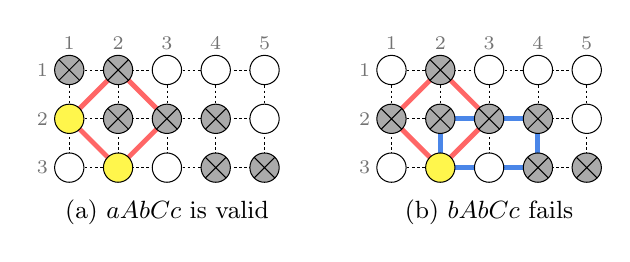
\begin{tikzpicture}[x=0.62cm,y=0.62cm,baseline=(current bounding box.north)]
  \begin{scope}[xshift=0.000cm]
    \draw[black,line width=0.25pt,dash pattern=on 0.93pt off 0.93pt] (1,-1) -- (5,-1) (1,-2) -- (5,-2) (1,-3) -- (5,-3) (1,-1) -- (1,-3) (2,-1) -- (2,-3) (3,-1) -- (3,-3) (4,-1) -- (4,-3) (5,-1) -- (5,-3);
    \draw[kred,line width=1.76pt,line join=round] (1,-2) -- (2,-1) -- (3,-2) -- (2,-3) -- cycle;
    \filldraw[fill=kgray,draw=black,line width=0.37pt] (1,-1) circle (0.3);
    \draw[black,line width=0.37pt] (0.788,-0.788) -- (1.212,-1.212) (0.788,-1.212) -- (1.212,-0.788);
    \filldraw[fill=kgray,draw=black,line width=0.37pt] (2,-1) circle (0.3);
    \draw[black,line width=0.37pt] (1.788,-0.788) -- (2.212,-1.212) (1.788,-1.212) -- (2.212,-0.788);
    \filldraw[fill=white,draw=black,line width=0.37pt] (3,-1) circle (0.3);
    \filldraw[fill=white,draw=black,line width=0.37pt] (4,-1) circle (0.3);
    \filldraw[fill=white,draw=black,line width=0.37pt] (5,-1) circle (0.3);
    \filldraw[fill=kyellow,draw=black,line width=0.37pt] (1,-2) circle (0.3);
    \filldraw[fill=kgray,draw=black,line width=0.37pt] (2,-2) circle (0.3);
    \draw[black,line width=0.37pt] (1.788,-1.788) -- (2.212,-2.212) (1.788,-2.212) -- (2.212,-1.788);
    \filldraw[fill=kgray,draw=black,line width=0.37pt] (3,-2) circle (0.3);
    \draw[black,line width=0.37pt] (2.788,-1.788) -- (3.212,-2.212) (2.788,-2.212) -- (3.212,-1.788);
    \filldraw[fill=kgray,draw=black,line width=0.37pt] (4,-2) circle (0.3);
    \draw[black,line width=0.37pt] (3.788,-1.788) -- (4.212,-2.212) (3.788,-2.212) -- (4.212,-1.788);
    \filldraw[fill=white,draw=black,line width=0.37pt] (5,-2) circle (0.3);
    \filldraw[fill=white,draw=black,line width=0.37pt] (1,-3) circle (0.3);
    \filldraw[fill=kyellow,draw=black,line width=0.37pt] (2,-3) circle (0.3);
    \filldraw[fill=white,draw=black,line width=0.37pt] (3,-3) circle (0.3);
    \filldraw[fill=kgray,draw=black,line width=0.37pt] (4,-3) circle (0.3);
    \draw[black,line width=0.37pt] (3.788,-2.788) -- (4.212,-3.212) (3.788,-3.212) -- (4.212,-2.788);
    \filldraw[fill=kgray,draw=black,line width=0.37pt] (5,-3) circle (0.3);
    \draw[black,line width=0.37pt] (4.788,-2.788) -- (5.212,-3.212) (4.788,-3.212) -- (5.212,-2.788);
    \node[lab] at (1,-0.45) {1};
    \node[lab] at (2,-0.45) {2};
    \node[lab] at (3,-0.45) {3};
    \node[lab] at (4,-0.45) {4};
    \node[lab] at (5,-0.45) {5};
    \node[lab] at (0.45,-1) {1};
    \node[lab] at (0.45,-2) {2};
    \node[lab] at (0.45,-3) {3};
    \node[capt,anchor=north] at (3.00,-3.45) {(a) $aAbCc$ is valid};
  \end{scope}
  \begin{scope}[xshift=4.092cm]
    \draw[black,line width=0.25pt,dash pattern=on 0.93pt off 0.93pt] (1,-1) -- (5,-1) (1,-2) -- (5,-2) (1,-3) -- (5,-3) (1,-1) -- (1,-3) (2,-1) -- (2,-3) (3,-1) -- (3,-3) (4,-1) -- (4,-3) (5,-1) -- (5,-3);
    \draw[kblue,line width=1.76pt,line join=round] (2,-2) -- (4,-2) -- (4,-3) -- (2,-3) -- cycle;
    \draw[kred,line width=1.76pt,line join=round] (1,-2) -- (2,-1) -- (3,-2) -- (2,-3) -- cycle;
    \filldraw[fill=white,draw=black,line width=0.37pt] (1,-1) circle (0.3);
    \filldraw[fill=kgray,draw=black,line width=0.37pt] (2,-1) circle (0.3);
    \draw[black,line width=0.37pt] (1.788,-0.788) -- (2.212,-1.212) (1.788,-1.212) -- (2.212,-0.788);
    \filldraw[fill=white,draw=black,line width=0.37pt] (3,-1) circle (0.3);
    \filldraw[fill=white,draw=black,line width=0.37pt] (4,-1) circle (0.3);
    \filldraw[fill=white,draw=black,line width=0.37pt] (5,-1) circle (0.3);
    \filldraw[fill=kgray,draw=black,line width=0.37pt] (1,-2) circle (0.3);
    \draw[black,line width=0.37pt] (0.788,-1.788) -- (1.212,-2.212) (0.788,-2.212) -- (1.212,-1.788);
    \filldraw[fill=kgray,draw=black,line width=0.37pt] (2,-2) circle (0.3);
    \draw[black,line width=0.37pt] (1.788,-1.788) -- (2.212,-2.212) (1.788,-2.212) -- (2.212,-1.788);
    \filldraw[fill=kgray,draw=black,line width=0.37pt] (3,-2) circle (0.3);
    \draw[black,line width=0.37pt] (2.788,-1.788) -- (3.212,-2.212) (2.788,-2.212) -- (3.212,-1.788);
    \filldraw[fill=kgray,draw=black,line width=0.37pt] (4,-2) circle (0.3);
    \draw[black,line width=0.37pt] (3.788,-1.788) -- (4.212,-2.212) (3.788,-2.212) -- (4.212,-1.788);
    \filldraw[fill=white,draw=black,line width=0.37pt] (5,-2) circle (0.3);
    \filldraw[fill=white,draw=black,line width=0.37pt] (1,-3) circle (0.3);
    \filldraw[fill=kyellow,draw=black,line width=0.37pt] (2,-3) circle (0.3);
    \filldraw[fill=white,draw=black,line width=0.37pt] (3,-3) circle (0.3);
    \filldraw[fill=kgray,draw=black,line width=0.37pt] (4,-3) circle (0.3);
    \draw[black,line width=0.37pt] (3.788,-2.788) -- (4.212,-3.212) (3.788,-3.212) -- (4.212,-2.788);
    \filldraw[fill=kgray,draw=black,line width=0.37pt] (5,-3) circle (0.3);
    \draw[black,line width=0.37pt] (4.788,-2.788) -- (5.212,-3.212) (4.788,-3.212) -- (5.212,-2.788);
    \node[lab] at (1,-0.45) {1};
    \node[lab] at (2,-0.45) {2};
    \node[lab] at (3,-0.45) {3};
    \node[lab] at (4,-0.45) {4};
    \node[lab] at (5,-0.45) {5};
    \node[lab] at (0.45,-1) {1};
    \node[lab] at (0.45,-2) {2};
    \node[lab] at (0.45,-3) {3};
    \node[capt,anchor=north] at (3.00,-3.45) {(b) $bAbCc$ fails};
  \end{scope}
\end{tikzpicture}
}
\caption{The diamond test. (a) In $aAbCc$ the diamond $D(1,1)$ shows $(1,2)$
and $(2,3)$. This pair has no rival, since $(1,3)$ is white. (b) In $bAbCc$ it
shows only $(2,3)$, and so does the blue rectangle. The window $bAb$ fails.}
\label{fig:diamond}
\end{minipage}
\end{figure}

\subsection{\texorpdfstring{The class $AC$}{The class AC}}

Set $G_{AC}(z)=\sum_{m\ge2}|AC_m|z^m$, and define $G_{AB}$ and $G_X$ in the same
way, where the sum for $G_X$ starts at $m=1$. Write $\Phi=1-3z$. The nonempty
singleton strings with a given first letter have the series $z/\Phi$, and so do
those with a given last letter.

\begin{proposition}[the class $AC$]\label{prop:threeGAC}
We have
\begin{equation}\label{eq:GAC}
G_{AC}(z)=\frac{z^2-4z^3+10z^4-8z^5-3z^6}{(1-3z)^3},
\end{equation}
and
\begin{equation}\label{eq:GACcoef}
|AC_m|=2(m-1)(3m+2)\,3^{m-5}\qquad(m\ge4).
\end{equation}
\end{proposition}

\begin{proof}
Write a word of the class as $UAVCW$ with singleton strings $U$, $V$, and $W$.
By Table~\ref{tab:windows} only the windows centered on $A$ and on $C$ matter.
Read $C$ as $b$ when it is a tip, and likewise $A$. Then the window $sAt$ fails
exactly for $st\in\{bb,bc,cb\}$, and $sCt$ fails exactly for
$st\in\{bb,ba,ab\}$. We count by the length of $V$.

If $V$ is empty, a nonempty $U$ must end in $a$ and a nonempty $W$ must start
with $c$. This case contributes $z^2(1+z/\Phi)^2$.

If $V$ is a single letter $t$, let $p_t$ be the number of letters allowed at the
end of $U$ and $q_t$ the number allowed at the start of $W$. Then
$(p_a,p_b,p_c)=(3,1,2)$ and $(q_a,q_b,q_c)=(2,1,3)$. The contribution is
\[
z^3\sum_t\Bigl(1+\frac{p_tz}{\Phi}\Bigr)\Bigl(1+\frac{q_tz}{\Phi}\Bigr)
=z^3\Bigl(3+\frac{12z}{\Phi}+\frac{13z^2}{\Phi^2}\Bigr).
\]

If $V$ has at least $2$ letters, its first letter and the last letter of $U$
form one of $6$ allowed pairs, or $U$ is empty and the first letter of $V$ is
free. This gives the factor $3+6z/\Phi$. The other end gives the same factor,
and the letters of $V$ between its first and last are free. The contribution
is $z^4(3+6z/\Phi)^2/\Phi=9z^4(1-z)^2/\Phi^3$.

Adding the $3$ cases gives~\eqref{eq:GAC}. Since
$[z^m]z^k\Phi^{-3}=\binom{m-k+2}23^{m-k}$, the coefficient of $z^m$ for $m\ge4$
is~\eqref{eq:GACcoef}.
\end{proof}

Let $E_m$ be the number of optima of the $3\times m$ grid with a column that is
black in rows $1$ and $3$ (\seqnum{A398448}). Such a column is $B$ or $X$. So
$E_m$ counts the optima in the $5$ classes other than $AC$ and $CA$, and
by~\eqref{eq:classsym},
\begin{equation}\label{eq:classsum}
a_3(m)=2|AC_m|+4|AB_m|+|X_m|=2|AC_m|+E_m\qquad(m\ge3).
\end{equation}

\subsection{\texorpdfstring{The classes $AB$ and $X$}{The classes AB and X}}\label{sec:threeruns}

Put $L=1-2z-2z^2$, $N=1+2z^2$, and $\Psi=LN=1-2z-4z^3-4z^4$. Call a singleton
string \emph{restricted} if it has no $2$ letters $b$ at distance $2$. In the
classes $AB$ and $X$ the windows $bsb$ fail, so every run of singletons is
restricted. Give the letter $b$ the type $1$ and the outer letters the type
$0$. For types $i$ and $j$, let $h_{ij}(z)$ count by length the strings
$y_1\cdots y_n$ with $n\ge0$ that can follow $2$ letters of types $i$ and $j$ in
a restricted string. Write $h_{ij}=h_{ij}^0+h_{ij}^1$, where $h_{ij}^\beta$
counts the strings whose last letter has type $\beta$, and the empty string is
given the type $j$. The letter $y_1$ can be $a$ or $c$, and it can be $b$ when
$i=0$. Hence, for $\beta\in\{0,1\}$,
\[
h_{ij}^\beta=[j=\beta]+2z\,h_{j0}^\beta+[i=0]\,z\,h_{j1}^\beta .
\]
Solving these $2$ linear systems gives
\begin{equation}\label{eq:hsol}
\begin{aligned}
\Psi h_{00}^0&=1+2z^2+2z^3,&\Psi h_{00}^1&=z+z^2,&\Psi h_{10}^0&=1,&\Psi h_{10}^1&=2z^2+2z^3,\\
\Psi h_{00}&=1+z+3z^2+2z^3,&\Psi h_{01}&=1+z,&\Psi h_{10}&=1+2z^2+2z^3,&\Psi h_{11}&=1.
\end{aligned}
\end{equation}

We read a run of singletons away from the double or triple next to it, as
$w_1w_2\cdots w_n$ with $n\ge1$. We need $4$ series for such runs. Let $g_0$
count the restricted runs whose first letter is a given outer letter, and
$g_1$ those with $w_1=b$. Let $u$ and $v$ count the same runs under the extra
condition that $w_2$, if present, is outer. A missing letter before $w_1$ acts
as a letter of type $0$, and the extra condition acts as a letter of type
$1$. Hence
\begin{equation}\label{eq:runs}
g_0=zh_{00},\qquad g_1=zh_{01},\qquad u=zh_{10},\qquad v=zh_{11}.
\end{equation}

\begin{proposition}[the class $X$]\label{prop:GX}
We have
\[
G_X(z)=z\bigl(1+4u+2v+2u^2+v^2\bigr)
=\frac{z(1+2z-7z^2-4z^3-2z^4-8z^5-4z^6)}{L^2N}.
\]
\end{proposition}

\begin{proof}
Write the word as $UXW$. Both runs are restricted. The failing windows $bsX$
and $Xsb$ of Table~\ref{tab:windows} say that the second letter from $X$ is
outer. The window centered on $X$ allows the neighbor pairs $ac$, $ca$, and
$bb$. So a run on one side only contributes $2u+v$, for either side, and
runs on both sides contribute $2u^2+v^2$. The second form follows
from~\eqref{eq:hsol} and~\eqref{eq:runs}.
\end{proof}

Now write a word of the class $AB$ as $UAVBW$. For a letter $t$ next to $A$ in
$V$, let $\ell_t$ count the strings $U$ that are allowed, including the empty
one. For a letter $t$ next to $B$ in $V$, let $r_t$ count the strings $W$ that
are allowed. By Table~\ref{tab:windows}, the window $bsA$ makes the second
letter of $U$ from $A$ outer, and nothing restricts the second letter of
$W$. The windows centered on $A$ allow the letters $a,b,c$ before $At$ for
$t=a$, only $a$ for $t=b$, and $a,c$ for $t=c$. The windows centered on $B$
allow only $c$ after $tB$ for $t=a$, the letters $b,c$ for $t=b$, and $a,b$
for $t=c$. Hence
\begin{equation}\label{eq:lr}
(\ell_a,\ell_b,\ell_c)=(1+2u+v,\ 1+u,\ 1+2u),\qquad
(r_a,r_b,r_c)=(1+g_0,\ 1+g_0+g_1,\ 1+g_0+g_1).
\end{equation}

\begin{proposition}[the class $AB$, $P_B$ by computer algebra]\label{prop:GAB}
With the series of~\eqref{eq:hsol} to~\eqref{eq:lr},
\begin{equation}\label{eq:GAB}
\begin{aligned}
G_{AB}(z)={}&z^2(1+2u)(1+g_0+g_1)+z^3(\ell_ar_a+\ell_br_b+\ell_cr_c)\\
&+z^4\sum_{\sigma\in\{0,1\}}\lambda_\sigma\bigl(h^0_{\sigma0}\,(r_a+r_c)+2h^1_{\sigma0}\,r_b\bigr),
\end{aligned}
\end{equation}
where $\lambda_0=\ell_a+\ell_c$ and $\lambda_1=\ell_b$. Moreover $G_{AB}=P_B/\Psi^3$
with
\begin{equation}\label{eq:PB}
P_B(z)=z^2(1+z)(1+z^2-3z^3+4z^6+4z^7).
\end{equation}
\end{proposition}

\begin{proof}
Let $k$ be the length of $V=v_1\cdots v_k$. For $k=0$ the windows $sAB$ and
$ABt$ of Table~\ref{tab:windows} require $s\ne b$ and $t\ne a$, which gives the
first term. For $k=1$ the window $Av_1B$ passes, and the windows centered on
$A$ and $B$ give $\ell_tr_t$ for $v_1=t$.

Let $k\ge2$. The window $Av_1v_2$ makes $v_2$ outer, and the window
$v_{k-1}v_kB$ passes. So $V$ is a restricted string whose second letter is
outer, and its weight is $\ell_{v_1}r_{v_k}$. Let $\sigma$ be the type of
$v_1$. Summing $\ell_{v_1}$ over the letters $v_1$ of type $\sigma$ gives
$\lambda_\sigma$. The string $v_3\cdots v_k$ follows $2$ letters of types
$\sigma$ and $0$. If it is empty, then $v_k=v_2$ is outer and the $2$ choices
give $r_a+r_c$. If it is not empty and $v_k$ is outer, there are $2$ choices
for $v_2$, and $h^0_{\sigma0}$ counts each string $v_3\cdots v_{k-1}$ twice,
once for each $v_k$. So the weight is again $h^0_{\sigma0}(r_a+r_c)$. If
$v_k=b$, the $2$ choices for $v_2$ give $2h^1_{\sigma0}r_b$. This
proves~\eqref{eq:GAB}. Substituting~\eqref{eq:hsol} and~\eqref{eq:runs} and
expanding gives~\eqref{eq:PB}.
\end{proof}

\subsection{Generating function, closed form, and asymptotics}

\begin{theorem}[three-row generating function, $P$ by computer algebra]\label{thm:threegf}
\leavevmode
\begin{enumerate}[(a)]
\item We have
\begin{equation}\label{eq:PQ}
\sum_{m\ge1}a_3(m)z^m=2G_{AC}+4G_{AB}+G_X=\frac{P(z)}{Q(z)},
\end{equation}
where $Q=(1-3z)^3(1-2z-2z^2)^3(1+2z^2)^3$ and
\begin{align*}
P(z)={}&z-3z^2-34z^3+228z^4-641z^5+1307z^6-2186z^7\\
&+2056z^8-236z^9-1060z^{10}+2584z^{11}-4264z^{12}\\
&-1440z^{13}+704z^{14}-1024z^{15}+2080z^{16}+2176z^{17}+384z^{18}.
\end{align*}
\item The polynomials $P$ and $Q$ are coprime. So $Q$ is the reduced denominator,
and $a_3(m)$ satisfies the linear recurrence of order $15$ with characteristic
polynomial $x^{15}Q(1/x)$ for $m\ge19$ and no recurrence of smaller order.
\item We have
\[
\sum_{m\ge3}E_mz^m=\frac{z^3\,P_E(z)}{(1-2z-2z^2)^3(1+2z^2)^3},
\]
where $P_E=43-90z+128z^2-344z^3+44z^4+80z^5+328z^6+1728z^7+1888z^8+2208z^9
+2016z^{10}+640z^{11}$.
\end{enumerate}
\end{theorem}

\begin{proof}
(a) For $m\ge3$ the coefficient of $z^m$ in $2G_{AC}+4G_{AB}+G_X$ is $a_3(m)$
by~\eqref{eq:classsum}. The coefficients of $z$ and $z^2$ are $1$ and $12$.
These are $a_3(1)$ and $a_3(2)=a_2(3)$, by Section~\ref{sec:setup} and
Theorem~\ref{thm:strip}. Bringing the $3$ series of
Propositions~\ref{prop:threeGAC}, \ref{prop:GX}, and~\ref{prop:GAB} to the common
denominator $Q$ gives $P$.

(b) The factors $\Phi$, $L$, and $N$ of $Q$ are irreducible and distinct. At
$z=\frac13$ only $G_{AC}$ has a pole, and the numerator of~\eqref{eq:GAC} takes
the value $\frac4{81}$ there. So the pole at $\frac13$ has order $3$. The remainders of
$P_B$ modulo $L$ and modulo $N$ are $\frac z2$ and $\frac14-\frac z2$. They are
not zero, so $G_{AB}$ has poles of order $3$ at the roots of $L$ and of $N$.
The series $G_X$ has poles of order at most $2$ there, and $G_{AC}$ has none.
Hence the series~\eqref{eq:PQ} has a pole of order $3$ at every root of $Q$, and
$P$ and $Q$ are coprime. The statement on recurrences follows, since
$\deg P=18$.

(c) By~\eqref{eq:classsum} the series is $4G_{AB}+G_X$ without its terms in
$z$ and $z^2$, which are $z+10z^2$.
\end{proof}

The polynomials $P$, $P_B$, and $P_E$ were expanded in exact arithmetic with
SymPy~\cite{sympy2017}.

Let $\rho=1+\sqrt3$ and $\sigma=1-\sqrt3$, so that $L=(1-\rho z)(1-\sigma z)$.

\begin{theorem}[the number of three-row optima, checked by computer algebra]\label{thm:threecount}
For every $m\ge4$,
\begin{equation}\label{eq:threecount}
a_3(m)=4(m-1)(3m+2)\,3^{m-5}+p_+(m)\,\rho^m+p_-(m)\,\sigma^m+(-2)^{\lfloor m/2\rfloor}\kappa(m),
\end{equation}
where
\[
432\,p_\pm(m)=(19\pm11\sqrt3)m^2+(61\pm41\sqrt3)m+104\pm28\sqrt3,
\]
and $\kappa(m)=(2m^2+41m-104)/216$ for even $m$ and
$\kappa(m)=(7m^2-32m-175)/432$ for odd $m$. The last $3$ terms are $E_m$, and
\begin{equation}\label{eq:Eclosed}
E_m=p_+(m)\,\rho^m+p_-(m)\,\sigma^m+(-2)^{\lfloor m/2\rfloor}\kappa(m)
\end{equation}
holds for every $m\ge2$. Moreover $E_m>0$,
\begin{equation}\label{eq:asymp1}
E_m\sim\frac{19+11\sqrt3}{432}\,m^2(1+\sqrt3)^m,\qquad
a_3(m)=\frac4{81}m^23^m-\frac4{243}(m+2)3^m+O\bigl(m^2(1+\sqrt3)^m\bigr),
\end{equation}
and the fraction of the $m^23^{m-1}$ candidates that are valid tends to
$\frac4{27}$.
\end{theorem}

\begin{proof}
By~\eqref{eq:classsum} and~\eqref{eq:GACcoef} we have
$a_3(m)=4(m-1)(3m+2)3^{m-5}+E_m$ for $m\ge4$. So it is enough to
prove~\eqref{eq:Eclosed}. By~\eqref{eq:classsum}, $E_m$ is the coefficient of
$z^m$ in $4G_{AB}+G_X$ for $m\ge3$. This also holds for $m=2$. Indeed the optima
of the $3\times2$ grid are the transposes of the optima of
Theorem~\ref{thm:strip}. They are the $12$ words of type~I or~II, and $10$ of
them contain $B$ or $X$. By Propositions~\ref{prop:GX} and~\ref{prop:GAB}, the
series $4G_{AB}+G_X$ has the denominator $L^3N^3$ of degree $12$ and a numerator
of degree $13$. So $E_m$ satisfies for $m\ge14$ the linear recurrence of order
$12$ with characteristic polynomial $x^{12}L(1/x)^3N(1/x)^3$. Its roots are
$\rho$, $\sigma$, and $\pm i\sqrt2$, each of multiplicity $3$. The right side
of~\eqref{eq:Eclosed} is a combination of $m^j\rho^m$, $m^j\sigma^m$, and
$m^j(\pm i\sqrt2)^m$ with $j\le2$, so it satisfies the same recurrence for all
$m$. The two sides agree for $2\le m\le13$, which we checked in exact
arithmetic. Hence they agree for all $m\ge2$.

We have $|\sigma|<1$ and $|(-2)^{\lfloor m/2\rfloor}\kappa(m)|=O(m^22^{m/2})$,
and $\sqrt2<\rho$. This gives the asymptotic form of $E_m$. The expansion of
$a_3(m)$ follows, since
$4(m-1)(3m+2)3^{m-5}=\frac4{81}m^23^m-\frac4{243}(m+2)3^m$. Finally $E_m>0$
because $Xa^{m-1}$ is an optimum by Corollary~\ref{cor:threevalue}, and
$E_2=10$.
\end{proof}

\subsection{Optima up to symmetry}

Let $o_3(m)$ be the number of optima of the $3\times m$ grid up to the row
reflection and the column reversal. Its first values for $m=3,\dots,8$ are
$15$, $58$, $227$, $864$, $3190$, and $11502$ (\seqnum{A401226}).

\begin{theorem}[three-row orbits]\label{thm:threeorbits}
Let $M=1-2z^2-2z^4$. Then
\begin{align*}
4\sum_{m\ge3}o_3(m)z^m={}&\sum_{m\ge3}a_3(m)z^m+z^3+\frac{4z^3(1+z^4+z^6)}{M\,(1+2z^4)}\\
&+\frac{2z^3(1-z)(1+5z+3z^2-3z^3)}{(1-3z^2)^2}.
\end{align*}
For even $m\ge4$ we have $o_3(m)=\frac14\bigl(a_3(m)+2m\,3^{m/2-2}\bigr)$.
\end{theorem}

\begin{proof}
By Burnside's lemma, $4o_3(m)$ is $a_3(m)$ plus the numbers of optima fixed by
the row reflection, the column reversal, and the half turn.

\emph{Row reflection.} A fixed word uses only $b$, $B$, and $X$. A candidate of
this kind is $b^iXb^j$. For $i\ge2$ the window $bbX$ fails, and for $j\ge2$ the
window $Xbb$ fails (Table~\ref{tab:windows}). So the only fixed optimum is
$bXb$, which gives the term $z^3$.

\emph{Column reversal.} A fixed word is a palindrome. A candidate has
different doubles, so a fixed candidate has the form $UXU^{\mathrm{rev}}$ and
$m$ is odd. The window centered on $X$ requires the last letter of $U$ to be
$b$. As in Proposition~\ref{prop:GX}, the allowed strings $U$ are counted by
$v$. This gives $z\,v(z^2)$.

\emph{Half turn.} It reverses the word and exchanges $a$ with $c$ and $A$ with
$C$. A fixed word of type~I is $UXU'$, where $U'$ is the image of $U$. The
neighbors of $X$ are then $ac$, $ca$, or $bb$, which are the allowed pairs. So
these words give $z\,(2u+v)(z^2)$. A fixed word of type~II has $A$ and $C$ in
mirror columns $j$ and $m+1-j$. Put $m=2k$ or $m=2k+1$, where in the second
case the middle letter is $b$. Take the class $AC$, so $j\le k$. The first $k$
letters determine the word. Only the windows centered on $A$ and $C$ can fail,
and these $2$ windows are mirror images. If $j=1$, the window on $A$ does not
exist or does not restrict the first $k$ letters, and there are $3^{k-1}$
words. If $j=k\ge2$, the right neighbor of $A$ is $C$ or the middle $b$, so the
left neighbor is $a$ and there are $3^{k-2}$ words. If $1<j<k$, there are
$6$ allowed pairs of neighbors and $2\cdot3^{k-2}$ words. The sum over $j$ is
$2k\,3^{k-2}$ for $k\ge2$. The class $CA$ has the same count. So type~II
gives $2$ fixed optima for $m=3$ and $4k\,3^{k-2}$ for $m\ge4$, with series
\[
2z^3+\tfrac49(1+z)\Bigl(\frac{3z^2}{(1-3z^2)^2}-3z^2\Bigr)
=\frac{2z^3(1-z)(1+5z+3z^2-3z^3)}{(1-3z^2)^2}.
\]

By~\eqref{eq:hsol} and~\eqref{eq:runs} the $2$ contributions of the words
$UXU^{\mathrm{rev}}$ and $UXU'$ add up to
$2z\,(u+v)(z^2)=4z^3(1+z^4+z^6)/\Psi(z^2)$, and $\Psi(z^2)=M(1+2z^4)$. For even
$m\ge4$ only the type~II words are fixed, and $4k\,3^{k-2}=2m\,3^{m/2-2}$.
\end{proof}

\section{Four rows}\label{sec:four}

Let $m\ge6$. Then $f(4,m)=m+4=m+q_4$ by Theorem~\ref{thm:imports}(c). So every
optimum is an axis-valid blackout with $m+q_4$ points, and
Theorem~\ref{thm:imports}(b) describes it. It has $4$ doubles and $m-4$
singletons, and the row pairs of the doubles are the $4$ edges of a $4$-cycle
on the rows. There are $3$ such cycles, one for each of the bipartitions
$\{1,2\}\mid\{3,4\}$, $\{1,3\}\mid\{2,4\}$, and $\{1,4\}\mid\{2,3\}$. A
\emph{candidate} is a word of singletons and doubles in which the doubles carry
each edge of one of these cycles exactly once. Its pair set $F$ is the edge set
of the cycle. There are $3\,(m)_4\,4^{m-4}$ candidates, where
$(m)_4=m(m-1)(m-2)(m-3)$. Every candidate is axis-valid, and it hides no
axis-aligned rectangle, since its doubles have different pairs. By
Lemma~\ref{lem:tilted-narrow}, each tilted rectangle has span at most $3$.

\subsection{Hidden rectangles and a bound by hand}

\begin{theorem}[no hidden rectangle]\label{thm:hidden}
For $m\ge4$, no valid blackout of the $4\times m$ grid hides a rectangle.
\end{theorem}

\begin{proof}
Suppose that a rectangle $R$ is hidden. We find two other rectangles
$R_1\ne R_2$ with $C(R)=C(R_1)\triangle C(R_2)$. By Lemma~\ref{lem:diff} they
have the same presentation, so the blackout is not valid. If $R$ is
axis-aligned with columns $x,y$, take a third column $w$ and let $R_1$ and $R_2$
have the rows of $R$ and the columns $\{x,w\}$ and $\{y,w\}$. For the tilted
rectangles, let $1\le i\le m-3$ and let $\mathsf Q_i$ be the axis-aligned
rectangle with corners $(i,2)$, $(i,3)$, $(i+3,2)$, and $(i+3,3)$. Writing a
rectangle for its corner set, we have
\begin{equation}\label{eq:fourxor}
\begin{gathered}
\kC_i=\kA_i\,\triangle\,\mathsf Q_i,\qquad \kE_i=\kB_i\,\triangle\,\mathsf Q_i,\\
D(i+1,1)=D(i,2)\,\triangle\,\kA_i,\qquad D(i+1,2)=D(i,1)\,\triangle\,\kE_i .
\end{gathered}
\end{equation}
Each of the $3$ sets in an identity is the symmetric difference of the other
$2$. The first line handles $\kA_i$, $\kB_i$, $\kC_i$, and $\kE_i$. For a
diamond $D(j,1)$ or $D(j,2)$, use the second line with $i=j-1$ if $j\ge2$, and
with $i=j$ if $j=1$. In the second case we need the column $j+3=4$, and
$m\ge4$.
\end{proof}

The condition $m\ge4$ is needed. On the $4\times3$ grid the blackout
$\{(1,2),(2,1),(3,2),(2,3)\}$ is valid and hides $D(1,1)$.

\begin{theorem}[forbidden-block bound]\label{thm:foursurvival}
For every $m\ge6$,
\[
a_4(m)\le3\,(m)_4\,4^{m-4}\Bigl(\frac{53}{64}\Bigr)^{k},\qquad
k=\max\bigl(0,\lfloor m/4\rfloor-4\bigr).
\]
Hence $a_4(m)=O\bigl(m^4\,212^{m/4}\bigr)$, and $212^{1/4}<3.816$.
\end{theorem}

\begin{proof}
Fix the pair set $F$ and the columns and pairs of the $4$ doubles. This can be
done in $3\,(m)_4$ ways. Call $4$ consecutive singleton columns a \emph{block},
and record it by the word of its $4$ black rows. We show that a block of an
optimum avoids at least $44$ of the $256$ words.

The \emph{template words} $2413$, $3412$, $2143$, and $3142$ are the rows of the
corners of $\kC_x$, $\kA_x$, $\kE_x$, and $\kB_x$, where $x$ is the first column
of the block. They are the permutations of $1234$ whose first and last letters
both lie in $\{2,3\}$. Let $\tau$ be one of these $4$ rectangles and
$t_1t_2t_3t_4$ its word.

First, the block is not a template word, since $\tau$ would be hidden
(Theorem~\ref{thm:hidden}). Second, the block is not obtained from
$t_1t_2t_3t_4$ by exchanging $t_p$ and $t_q$. In that case $\tau$ would show
exactly its corners $(x+p-1,t_p)$ and $(x+q-1,t_q)$, and so would the
axis-aligned rectangle through these $2$ points. The words obtained by such
exchanges are the templates and the $16$ permutations with exactly one of the
first and last letters in $\{2,3\}$. So $20$ permutations are excluded.

Third, the block is not obtained from $t_1t_2t_3t_4$ by changing one letter
$t_p=r$ to a letter $s$ with $\{r,s\}\in F$. In that case $\tau$ would show only
$(x+p-1,r)$. Let $d$ be the double column with the pair $\{r,s\}$. The
axis-aligned rectangle on the rows $r,s$ and the columns $x+p-1$ and $d$ would
also show only $(x+p-1,r)$. Each row lies in $2$ pairs of $F$, so each template
gives $8$ such words. They repeat a letter, so they are not permutations.
Two templates can give the same word only if they differ by exchanging $2$
letters $r,s$ with $\{r,s\}\in F$, and then they share $2$ words. The $4$ pairs
of templates that differ by one exchange use the letters $\{2,3\}$ twice and
$\{1,4\}$ twice. So at least $32-8=24$ further words are excluded, and a block
has at most $256-20-24=212=4^4\cdot\frac{53}{64}$ words.

Cut the columns into the $\lfloor m/4\rfloor$ groups $4j-3,\ldots,4j$. At most
$4$ groups contain a double, so at least $k$ groups are blocks. Every other
singleton column has at most $4$ choices. This gives the bound.
\end{proof}

\subsection{The automaton}

\begin{lemma}[six columns of memory]\label{lem:fourmemory}
Let $m\ge6$. A candidate of the $4\times m$ grid is an optimum if and only if
\begin{enumerate}[(i)]
\item no tilted rectangle is hidden,
\item no tilted rectangle that shows $1$ or $2$ corners has a rival in the sense
of Lemma~\ref{lem:rival}, and
\item no $2$ distinct tilted rectangles that lie in $7$ consecutive columns have
the same presentation.
\end{enumerate}
\end{lemma}

\begin{proof}
An optimum is valid, so (ii) and (iii) hold, and (i) holds by
Theorem~\ref{thm:hidden}. Conversely, let a candidate satisfy (i) to (iii), and
suppose that $2$ distinct rectangles have the same presentation $P$. They are not
both axis-aligned, since a candidate is axis-valid. If $P$ is empty, both
are hidden. One of them is tilted, which contradicts (i). So $P$ is not empty,
and $|P|\le2$ by Lemma~\ref{lem:threecorners}. If one rectangle is
axis-aligned, it is a rival of $P$, which contradicts (ii). If both are tilted,
choose a column $c$ that meets $P$. Both rectangles have a corner in column $c$
and span at most $3$, so they lie in the columns $c-3$ to $c+3$. This
contradicts (iii). Hence the candidate is valid. It has $m+4$ points, so it is
an optimum.
\end{proof}

By Lemma~\ref{lem:rival}, whether a set $P$ of $1$ or $2$ white points has a
rival depends only on $F$ and on the letters of the columns that meet $P$. So
the $3$ conditions can be tested while the word is read from left to right.

\begin{proposition}[the automaton]\label{prop:fourautomaton}
Let $F$ be the edge set of a $4$-cycle on the rows. The automaton $\mathcal A_F$
reads words in the $4$ singleton letters and the $4$ pairs of $F$. A state
$(u,U)$ records the last $6$ letters $u$ (all letters, if fewer than $6$ have
been read) and the set $U\subseteq F$ of pairs read so far. The start state is
the empty word with $U=\emptyset$. On reading a letter $y$, the automaton
rejects if $y\in U$, or if some tilted rectangle in the word $uy$ that has a
corner in the new column
\begin{enumerate}[(1)]
\item is hidden, or
\item shows $1$ or $2$ corners and has a rival, or
\item has the same presentation as another tilted rectangle in $uy$.
\end{enumerate}
Otherwise it moves to the state given by $uy$ and $U\cup(\{y\}\cap F)$. A word
is accepted if it is read to the end without rejection and the final state has
$U=F$. For each $m\ge6$, the accepted words of length $m$ are exactly the optima
of the $4\times m$ grid with pair set $F$.
\end{proposition}

\begin{proof}
An accepted word contains each pair of $F$ exactly once, so it is a candidate
with pair set $F$. A tilted rectangle has span at most $3$. When its last
column is read, it lies in the last $4$ letters of $uy$, and it is tested for
(1) and (2). Two tilted rectangles in $7$ consecutive columns both lie in $uy$
when the later of their last columns is read, and they are compared in (3). So
an accepted word of length $m\ge6$ satisfies the conditions of
Lemma~\ref{lem:fourmemory} and is an optimum. Conversely, an optimum with pair
set $F$ is a candidate, so no pair is read twice and the final state has $U=F$.
It satisfies the conditions of Lemma~\ref{lem:fourmemory}, so no step rejects.
\end{proof}

\subsection{The generating function and the growth rate}

The statements of this subsection are computer-assisted. We built
$\mathcal A_F$ for the $3$ pair sets. The automata have $60975$, $138095$, and
$55575$ states. For each we also have a smaller machine from an earlier search,
with $2519$, $3089$, and $2119$ reachable states, and a program checks that it
accepts the same words as $\mathcal A_F$. Two separately written transfer
counters give the same counts for all $m\le1500$. For $m\le10$ the counts also
agree with a test of every candidate against the definition. At $m=12$ the
pair sets of $\{1,2\}\mid\{3,4\}$, $\{1,3\}\mid\{2,4\}$, and $\{1,4\}\mid\{2,3\}$
give $114424$, $1785768$, and $137656$ optima.


\begin{theorem}[four-row generating function, computer-assisted]\label{thm:fourgfexact}
There are coprime integer polynomials $P_4=26z^6-826z^7+\cdots$ of degree $444$
and $Q_4$ of degree $420$ with $Q_4(0)=1$ and
\[
\sum_{m\ge6}a_4(m)z^m=\frac{P_4(z)}{Q_4(z)}.
\]
Write $Q_4=\sum_jq_jz^j$. The recurrence $\sum_{j=0}^{420}q_j\,a_4(n-j)=0$ holds for
every $n\ge445$ and fails at $n=444$. Over the integers,
\[
Q_4=(1-z)^2(1+z)^2\,g_5^3\,\tilde g_5^3\,g_6^3\,g_{11}^5\,g_{17}^3\,g_{19}^3\,g_{20}^5\,g_{21}^5,
\]
where $g_d$ and $\tilde g_d$ are irreducible of degree $d$ with constant term $1$.
Here $g_5=1+3z^2-2z^3+2z^4-z^5$, $\tilde g_5=1+z^2-z^5$,
$g_6=1-z^2-z^5-2z^6$, and
\begin{align*}
g_{20}={}&1-4z+2z^2+z^3-3z^4+5z^5+z^6-3z^7+7z^8+2z^9+30z^{10}-7z^{11}+10z^{12}\\
&+12z^{13}+2z^{14}+17z^{15}+26z^{16}+19z^{17}-26z^{18}-4z^{19}+8z^{20}.
\end{align*}
\end{theorem}

\begin{proof}
By Proposition~\ref{prop:fourautomaton}, $a_4(m)$ is the number of words of
length $m$ accepted by the $3$ automata. We computed $a_4(m)$ for $m\le1500$,
and the Berlekamp--Massey algorithm, run modulo $8$ primes, produced $P_4$ and
$Q_4$. This is only a guess, so we certify it. For each pair set let $M_F$ be the
transfer matrix of the smaller machine and $v_F(n)=v_F(0)M_F^n$ its vector of
state counts after $n$ letters. The programs check the vector identity
$\sum_jq_j\,v_F(n_F-j)=0$ in exact integer arithmetic, with $n_F=436$, $435$, and
$445$ for the $3$ pair sets. Multiplying by powers of $M_F$ gives the same
identity at every larger index. Since $a_4(n)$ is a fixed linear function of the
vectors $v_F(n)$, the recurrence holds for all $n\ge445$. Then $P_4$ is the
product of $Q_4$ and the series, cut off after degree $444$. Its coefficient of
$z^{444}$ is not zero, so the recurrence fails at $444$. The factorization and
the coprimality were computed with SymPy~\cite{sympy2017}.
\end{proof}

The other factors of $Q_4$ and the coefficients of $P_4$ are in the file
\nolinkurl{four_row_recurrence.json} of the repository~\cite{repo} and in the
OEIS entry \seqnum{A401224}. The $3$ pair sets have rational series of their
own, with reduced denominators of degrees $162$, $153$, and $107$. The factor
$g_{20}$ occurs only for the pair set of $\{1,3\}\mid\{2,4\}$.

\begin{corollary}[growth, computer-assisted]\label{cor:fourgrowth}
Let $\rho_4=3.351996777310\ldots$ be the largest real root of
$x^{20}g_{20}(1/x)$. There is a polynomial $\pi$ of degree $4$ with
$a_4(m)=\rho_4^m\,\pi(m)+O\bigl((1000/341)^m\bigr)$. Hence
$a_4(m)\sim c\,m^4\rho_4^m$ with $c=8.16109707\ldots\times10^{-5}$, and almost all
optima have the pair set of $\{1,3\}\mid\{2,4\}$.
\end{corollary}

\begin{proof}
We isolate the complex roots of every factor of $Q_4$ with exact rational
bounds. The only root of modulus at most $0.341$ is $r=1/\rho_4=0.29832\ldots$.
It is a simple root of $g_{20}$, so it is a pole of order $5$ of $P_4/Q_4$,
because $P_4$ and $Q_4$ are coprime. Write
$P_4/Q_4=\sum_{j=1}^{5}c_j(1-z/r)^{-j}+T(z)$ with $c_5\ne0$. The series $T$
has no pole of modulus at most $0.341$, so its coefficients are
$O((1000/341)^m)$. Since $[z^m](1-z/r)^{-j}=\rho_4^m\binom{m+j-1}{j-1}$, we get
$\pi(m)=\sum_jc_j\binom{m+j-1}{j-1}$ and $c=c_5/24$. Interval arithmetic gives
$8.1610970775\times10^{-5}<c<8.1610970776\times10^{-5}$. The last claim holds
because $g_{20}$ does not divide the denominators of the other $2$ pair sets.
\end{proof}

\section{Five rows}\label{sec:five}

Let $m\ge8$. By Theorem~\ref{thm:imports}, $f(5,m)=m+6$, and an optimum has $6$
doubles, whose row pairs are the edges of a complete bipartite graph with parts
of sizes $2$ and $3$, and $m-6$ singletons. Table~\ref{tab:fivevalues} lists the
number of optima for $8\le m\le23$ (\seqnum{A401225}). These values are
computer-assisted. Two separately written transfer counters over the columns
agree for $13\le m\le23$, and for $8\le m\le12$ the values agree with complete
enumerations (Section~\ref{sec:verify}).

\begin{table}[!htb]
\centering\footnotesize\setlength{\tabcolsep}{5pt}
\begin{tabular}{@{}rr@{\hspace{2.5em}}rr@{\hspace{2.5em}}rr@{\hspace{2.5em}}rr@{}}
\toprule
$m$ & $a_5(m)$ & $m$ & $a_5(m)$ & $m$ & $a_5(m)$ & $m$ & $a_5(m)$\\
\midrule
$8$ & $4$ & $12$ & $24706$ & $16$ & $52128242$ & $20$ & $45743165894$\\
$9$ & $44$ & $13$ & $193406$ & $17$ & $299349210$ & $21$ & $230934909328$\\
$10$ & $350$ & $14$ & $1346758$ & $18$ & $1653637492$ & $22$ & $1139486126866$\\
$11$ & $3004$ & $15$ & $8650416$ & $19$ & $8828301226$ & $23$ & $5510071794736$\\
\bottomrule
\end{tabular}
\caption{The number of optima of the $5\times m$ grid (computer-assisted).}
\label{tab:fivevalues}
\end{table}

\section{Every fixed height}\label{sec:height}

Fix the height $h$. The letters are now all subsets of $\{1,\dots,h\}$, and a
blackout of the $h\times m$ grid is the column word $w=B_1\cdots B_m$. Write
$|w|=m$ for its length and $S(w)$ for the blackout. Let $\mathcal L_h$ be the
set of words of valid blackouts, of all lengths.

\begin{theorem}[regularity]\label{thm:regular}
For every $h\ge1$ the language $\mathcal L_h$ is regular. Hence the series
$\sum_{w\in\mathcal L_h}z^{|w|}u^{|S(w)|}$ is a rational function of $z$ and $u$.
\end{theorem}

\begin{proof}
The \emph{trace} of a rectangle of the $h\times m$ grid is the word
$Y_1\cdots Y_m$, where $Y_i$ is the set of rows of its corners in column $i$.
Different rectangles have different traces. By Lemma~\ref{lem:diff}, the word
$w$ is not valid if and only if there are $2$ different traces $Y$ and $Y'$ of
length $m$ with $Y_i\triangle Y'_i\subseteq B_i$ for every $i$.

The traces of all lengths form a regular language. The trace of an axis-aligned
rectangle is a letter $\{r,s\}$ with $r\ne s$, then some empty letters, then the
same letter again, with any number of empty letters before and after. By
Lemmas~\ref{lem:leftmost} and~\ref{lem:span}, the trace of a tilted rectangle is
one of finitely many words of length at most $W_h+1$, again with empty letters
before and after.

Read a triple $(w,Y,Y')$ of words of the same length as one word whose letters
are triples of sets. The triples in which $Y$ and $Y'$ are different traces and
$Y_i\triangle Y'_i\subseteq B_i$ for every $i$ form a regular language.
Forgetting $Y$ and $Y'$ keeps it regular. So the words that are not valid form
a regular language, and $\mathcal L_h$ is its complement.

Take a deterministic automaton for $\mathcal L_h$ and give the step that reads
$B$ the weight $zu^{|B|}$. Let $T(z,u)$ be the matrix of these weights, $\alpha$
the indicator row vector of the start state, and $\beta$ the indicator column
vector of the accepting states. Each word of $\mathcal L_h$ has exactly $1$
accepting path, so the series is $\alpha(I-T(z,u))^{-1}\beta$. This is rational
by Cramer's rule~\cite[Proposition~V.6]{flajolet2009}.
\end{proof}

\begin{theorem}[fixed height]\label{thm:rational}
Let $h\ge1$. The column words of the optima of the grids with $h$ rows form a
regular language, and $\sum_{m\ge1}a_h(m)z^m$ is a rational function.
\end{theorem}

\begin{proof}
For $h=1$ every blackout is valid, and $a_1(m)=1$. For $h=2$ the optima are
described in Theorem~\ref{thm:strip}, and the series is $z/(1-2z)^2$ up to its
first $2$ terms. Let $h\ge3$. By Theorem~\ref{thm:imports}(d) we have
$f(h,m)=m+q_h$ for all $m\ge m_h$. So $f(h,m)-m$ is eventually constant. Changing finitely many words keeps a language regular and changes the
series by a polynomial. It is therefore enough to treat the language
$\mathcal L_{h,q_h}$, where $\mathcal L_{h,k}$ is the set of words
$w\in\mathcal L_h$ with $|S(w)|-|w|=k$.

Put $e(w)=|S(w)|-|w|$, so that $e(uv)=e(u)+e(v)$. Every factor $v$ of a valid
word is the word of a valid blackout of a smaller grid. If $|v|\ge3$, then
$e(v)\le q_h$ by Theorem~\ref{thm:imports}(a). If $|v|\le2$, then
$e(v)\le2h-2$. Put $c_h=\max(q_h,2h-2)$. Now let $w=uv$ be valid with
$e(w)=k$. Then
\[
k-c_h\le e(u)=k-e(v)\le c_h .
\]
So an automaton for $\mathcal L_h$ can also keep the value $e(u)$ of the prefix
read so far. It rejects when this value leaves the interval $[k-c_h,c_h]$, and
at the end it accepts when the value is $k$. This is a finite automaton for
$\mathcal L_{h,k}$. The series of a regular language is rational, as in the
proof of Theorem~\ref{thm:regular}.
\end{proof}

The regularity of $\mathcal L_{h,q_h}$ also follows from a result of Guilhot,
Little, and Parkinson~\cite[Theorem~1(3)]{glp2025} on additive weights that are
bounded above on a regular language. Here the weight is $e$.

\section{Computations and verification}\label{sec:verify}

The code and the stored results are in the repository~\cite{repo}. From its
root, the scripts are in \nolinkurl{jis/scripts} and the evidence files in
\nolinkurl{jis/data}, and \nolinkurl{jis/scripts/README.md} gives the commands.
Every computed count has $2$ separately written checks, except $a_7(8)\ge18$.

\paragraph{Three rows.} The proofs in Section~\ref{sec:three} are by hand up to
the expansion of rational functions, which we did with SymPy~\cite{sympy2017}.
One program finds all optima of the
$3\times m$ grid from Definition~\ref{def:valid} for $m\le10$, and its counts
agree with~\eqref{eq:PQ}. A transfer matrix built from Table~\ref{tab:windows}
agrees with~\eqref{eq:PQ} and~\eqref{eq:Eclosed} for $m\le100$. For
Theorem~\ref{thm:threeorbits}, the fixed words are listed for $m\le24$ and the
orbits for $m\le10$. The files are \nolinkurl{three_row_*.json}.

\paragraph{Four rows.} A second certificate for Theorem~\ref{thm:fourgfexact} treats each pair set alone. It
checks the recurrence of that pair set on as many consecutive widths as the
machine has states, which is enough by the Cayley--Hamilton theorem. The files
are \nolinkurl{four_row_*.json}.

\paragraph{Five rows and small grids.} The files for
Proposition~\ref{prop:fivecounts} are \nolinkurl{five_row_count_*.json} and
\nolinkurl{five_row_optima_dp_w*.json}, and those for the other counts of
Table~\ref{tab:values} are in \nolinkurl{table_counts}. The SAT enumerations use
PySAT~\cite{pysat2018}. Each blackout found is tested again against
Definition~\ref{def:valid}.

\paragraph{Formal proofs.} The folder \nolinkurl{lean} of the repository
contains proofs in Lean of Lemmas~\ref{lem:diff}, \ref{lem:threecorners},
\ref{lem:span}, and~\ref{lem:girth}, of the Strip Theorem with its count, and of
the example after Theorem~\ref{thm:hidden}.

\section{Open questions}\label{sec:open}

\begin{enumerate}[(1),leftmargin=*]
\item What is the rational series $\sum_m a_5(m)z^m$, and what is the growth rate
of $a_5(m)$?
\item Is $a_h(m)\sim c_h\,m^{q_h}\rho_h^m$ for every $h$, as it is for $2\le h\le4$?
\item Remark~\ref{cor:oeisconj} settles the largest entry in each row of
\seqnum{A338885}. Is its smallest entry in row $n$ equal to
\seqnum{A228286}$(n)$, as conjectured there?
\end{enumerate}

\section{Acknowledgments}\label{sec:ack}

I thank Peter Kagey for posing the problem, and for discussing its early stages
with me, including the uniqueness of the $5\times5$ optimum and the first
graph-theoretic approach to the narrow grids. The design of Figure~\ref{fig:game} follows the figure in his posting of
Problem 001~\cite{kagey001}.


\bibliographystyle{jis}
\bibliography{enumeration}

\noindent 2020 {\it Mathematics Subject Classification}: Primary 05A15; Secondary
05A16, 05B40, 52C05, 68Q45, 68R15.

\noindent \emph{Keywords:} blackout, lattice rectangle, rational generating function,
transfer matrix, finite automaton, regular language.

\noindent (Concerned with sequences
\seqnum{A001787},
\seqnum{A002620},
\seqnum{A033638},
\seqnum{A228286},
\seqnum{A322284},
\seqnum{A338885},
\seqnum{A397315},
\seqnum{A398321},
\seqnum{A398448},
\seqnum{A399580},
\seqnum{A401223},
\seqnum{A401224},
\seqnum{A401225}, and
\seqnum{A401226}.)

\end{document}
